% Options for packages loaded elsewhere
\PassOptionsToPackage{unicode}{hyperref}
\PassOptionsToPackage{hyphens}{url}
%
\documentclass[
]{article}
\usepackage{amsmath,amssymb}
\usepackage{iftex}
\ifPDFTeX
  \usepackage[T1]{fontenc}
  \usepackage[utf8]{inputenc}
  \usepackage{textcomp} % provide euro and other symbols
\else % if luatex or xetex
  \usepackage{unicode-math} % this also loads fontspec
  \defaultfontfeatures{Scale=MatchLowercase}
  \defaultfontfeatures[\rmfamily]{Ligatures=TeX,Scale=1}
\fi
\usepackage{lmodern}
\ifPDFTeX\else
  % xetex/luatex font selection
\fi
% Use upquote if available, for straight quotes in verbatim environments
\IfFileExists{upquote.sty}{\usepackage{upquote}}{}
\IfFileExists{microtype.sty}{% use microtype if available
  \usepackage[]{microtype}
  \UseMicrotypeSet[protrusion]{basicmath} % disable protrusion for tt fonts
}{}
\makeatletter
\@ifundefined{KOMAClassName}{% if non-KOMA class
  \IfFileExists{parskip.sty}{%
    \usepackage{parskip}
  }{% else
    \setlength{\parindent}{0pt}
    \setlength{\parskip}{6pt plus 2pt minus 1pt}}
}{% if KOMA class
  \KOMAoptions{parskip=half}}
\makeatother
\usepackage{xcolor}
\usepackage[margin=1in]{geometry}
\usepackage{color}
\usepackage{fancyvrb}
\newcommand{\VerbBar}{|}
\newcommand{\VERB}{\Verb[commandchars=\\\{\}]}
\DefineVerbatimEnvironment{Highlighting}{Verbatim}{commandchars=\\\{\}}
% Add ',fontsize=\small' for more characters per line
\usepackage{framed}
\definecolor{shadecolor}{RGB}{248,248,248}
\newenvironment{Shaded}{\begin{snugshade}}{\end{snugshade}}
\newcommand{\AlertTok}[1]{\textcolor[rgb]{0.94,0.16,0.16}{#1}}
\newcommand{\AnnotationTok}[1]{\textcolor[rgb]{0.56,0.35,0.01}{\textbf{\textit{#1}}}}
\newcommand{\AttributeTok}[1]{\textcolor[rgb]{0.13,0.29,0.53}{#1}}
\newcommand{\BaseNTok}[1]{\textcolor[rgb]{0.00,0.00,0.81}{#1}}
\newcommand{\BuiltInTok}[1]{#1}
\newcommand{\CharTok}[1]{\textcolor[rgb]{0.31,0.60,0.02}{#1}}
\newcommand{\CommentTok}[1]{\textcolor[rgb]{0.56,0.35,0.01}{\textit{#1}}}
\newcommand{\CommentVarTok}[1]{\textcolor[rgb]{0.56,0.35,0.01}{\textbf{\textit{#1}}}}
\newcommand{\ConstantTok}[1]{\textcolor[rgb]{0.56,0.35,0.01}{#1}}
\newcommand{\ControlFlowTok}[1]{\textcolor[rgb]{0.13,0.29,0.53}{\textbf{#1}}}
\newcommand{\DataTypeTok}[1]{\textcolor[rgb]{0.13,0.29,0.53}{#1}}
\newcommand{\DecValTok}[1]{\textcolor[rgb]{0.00,0.00,0.81}{#1}}
\newcommand{\DocumentationTok}[1]{\textcolor[rgb]{0.56,0.35,0.01}{\textbf{\textit{#1}}}}
\newcommand{\ErrorTok}[1]{\textcolor[rgb]{0.64,0.00,0.00}{\textbf{#1}}}
\newcommand{\ExtensionTok}[1]{#1}
\newcommand{\FloatTok}[1]{\textcolor[rgb]{0.00,0.00,0.81}{#1}}
\newcommand{\FunctionTok}[1]{\textcolor[rgb]{0.13,0.29,0.53}{\textbf{#1}}}
\newcommand{\ImportTok}[1]{#1}
\newcommand{\InformationTok}[1]{\textcolor[rgb]{0.56,0.35,0.01}{\textbf{\textit{#1}}}}
\newcommand{\KeywordTok}[1]{\textcolor[rgb]{0.13,0.29,0.53}{\textbf{#1}}}
\newcommand{\NormalTok}[1]{#1}
\newcommand{\OperatorTok}[1]{\textcolor[rgb]{0.81,0.36,0.00}{\textbf{#1}}}
\newcommand{\OtherTok}[1]{\textcolor[rgb]{0.56,0.35,0.01}{#1}}
\newcommand{\PreprocessorTok}[1]{\textcolor[rgb]{0.56,0.35,0.01}{\textit{#1}}}
\newcommand{\RegionMarkerTok}[1]{#1}
\newcommand{\SpecialCharTok}[1]{\textcolor[rgb]{0.81,0.36,0.00}{\textbf{#1}}}
\newcommand{\SpecialStringTok}[1]{\textcolor[rgb]{0.31,0.60,0.02}{#1}}
\newcommand{\StringTok}[1]{\textcolor[rgb]{0.31,0.60,0.02}{#1}}
\newcommand{\VariableTok}[1]{\textcolor[rgb]{0.00,0.00,0.00}{#1}}
\newcommand{\VerbatimStringTok}[1]{\textcolor[rgb]{0.31,0.60,0.02}{#1}}
\newcommand{\WarningTok}[1]{\textcolor[rgb]{0.56,0.35,0.01}{\textbf{\textit{#1}}}}
\usepackage{graphicx}
\makeatletter
\def\maxwidth{\ifdim\Gin@nat@width>\linewidth\linewidth\else\Gin@nat@width\fi}
\def\maxheight{\ifdim\Gin@nat@height>\textheight\textheight\else\Gin@nat@height\fi}
\makeatother
% Scale images if necessary, so that they will not overflow the page
% margins by default, and it is still possible to overwrite the defaults
% using explicit options in \includegraphics[width, height, ...]{}
\setkeys{Gin}{width=\maxwidth,height=\maxheight,keepaspectratio}
% Set default figure placement to htbp
\makeatletter
\def\fps@figure{htbp}
\makeatother
\setlength{\emergencystretch}{3em} % prevent overfull lines
\providecommand{\tightlist}{%
  \setlength{\itemsep}{0pt}\setlength{\parskip}{0pt}}
\setcounter{secnumdepth}{-\maxdimen} % remove section numbering
\ifLuaTeX
  \usepackage{selnolig}  % disable illegal ligatures
\fi
\IfFileExists{bookmark.sty}{\usepackage{bookmark}}{\usepackage{hyperref}}
\IfFileExists{xurl.sty}{\usepackage{xurl}}{} % add URL line breaks if available
\urlstyle{same}
\hypersetup{
  pdftitle={Crypto\_EDA\_FE},
  pdfauthor={Yogesh Sahu},
  hidelinks,
  pdfcreator={LaTeX via pandoc}}

\title{Crypto\_EDA\_FE}
\author{Yogesh Sahu}
\date{01/05/2024}

\begin{document}
\maketitle

\hypertarget{introduction}{%
\section{Introduction}\label{introduction}}

\emph{Cryptocurrencies have emerged as a significant player in the
global financial landscape, with Bitcoin and Ethereum leading the pack.
Understanding the intricate dynamics of these digital assets is
paramount for investors, traders, and analysts alike. This report
embarks on a comprehensive analysis journey, employing exploratory data
analysis (EDA) and feature engineering (FE) techniques to gain profound
insights into cryptocurrency price movements and market behavior.}

\hypertarget{step-1-loading-and-preprocessing-historical-data}{%
\subparagraph{Step 1: Loading and Preprocessing Historical
Data}\label{step-1-loading-and-preprocessing-historical-data}}

The analysis initiates with the ingestion of historical cryptocurrency
data. Through meticulous preprocessing and data wrangling techniques, we
extract relevant information based on price action. This includes
crucial steps such as handling missing values, standardizing data
formats, and merging datasets to enrich the analytical scope.

\hypertarget{step-2-uncovering-trends-and-patterns}{%
\subparagraph{Step 2: Uncovering Trends and
Patterns}\label{step-2-uncovering-trends-and-patterns}}

Once the data is prepared, we delve into exploratory data analysis (EDA)
to uncover underlying trends, patterns, and relationships. While basic
visualizations provide initial insights, we'll leverage advanced
techniques such as feature engineering to extract more meaningful
information from the data. Utilizing visualizations and statistical
summaries, we aim to unravel the complex dynamics of cryptocurrency
markets. This includes identifying cyclical trends, seasonal patterns,
and anomalous behavior that may impact investment decisions.

\hypertarget{step-3-investigating-halving-events}{%
\subparagraph{Step 3: Investigating Halving
Events}\label{step-3-investigating-halving-events}}

A crucial aspect of our analysis involves investigating the impact of
halving events on cryptocurrency prices. Halving events, which occur at
predetermined intervals for certain cryptocurrencies like Bitcoin, have
historically influenced market dynamics. By examining price action
surrounding these events, we seek to discern their implications for
market sentiment and investor behavior.

\hypertarget{step-4-market-cap-segmentation}{%
\subparagraph{Step 4: Market Cap
Segmentation}\label{step-4-market-cap-segmentation}}

In addition to price movements, we delve into market cap segmentation to
gain insights into the distribution of value across different
cryptocurrencies. This segmentation provides a nuanced understanding of
market dynamics, highlighting the relative prominence of various digital
assets within the cryptocurrency ecosystem.

\hypertarget{advanced-visualization-and-model-preparation}{%
\paragraph{Advanced Visualization and Model
Preparation}\label{advanced-visualization-and-model-preparation}}

Moving beyond basic visualizations, we will employ advanced
visualization techniques to gain deeper insights into the data.
Furthermore, leveraging the feature-engineered dataset, we will prepare
the groundwork for developing robust machine learning (ML) and deep
learning (DL) models. These models will utilize the enriched dataset to
predict cryptocurrency price movements and aid in making informed
investment decisions.

By combining advanced visualization techniques with feature engineering
and model preparation, this report aims to provide a comprehensive
understanding of cryptocurrency markets. These insights will not only
facilitate informed decision-making but also serve as a solid foundation
for building predictive models that can further enhance investment
strategies and opportunities in the cryptocurrency space.

\hypertarget{load-data-and-extract-data-based-on-price-action-analysis}{%
\section{Load Data and Extract Data Based on Price Action
Analysis}\label{load-data-and-extract-data-based-on-price-action-analysis}}

\hypertarget{data-prep---adding-returns-log-returns}{%
\subsection{Data Prep - Adding Returns / log
Returns}\label{data-prep---adding-returns-log-returns}}

This section provides context for the code snippet, indicating that it
focuses on preprocessing cryptocurrency data and engineering features to
enhance the analysis process. The subsequent code demonstrates loading
data, merging datasets, and creating new columns to capture
\texttt{percentage\ change\ and\ logarithmic\ return}, essential metrics
for understanding cryptocurrency price movements.

\begin{Shaded}
\begin{Highlighting}[]
\NormalTok{df\_pa }\OtherTok{\textless{}{-}}\NormalTok{ df }\SpecialCharTok{\%\textgreater{}\%}
  \FunctionTok{select}\NormalTok{(date,id,slug,open, close,market\_cap,rank) }\SpecialCharTok{\%\textgreater{}\%}
  \FunctionTok{mutate}\NormalTok{(}
    \AttributeTok{pct\_change =}\NormalTok{ (close }\SpecialCharTok{{-}}\NormalTok{ open) }\SpecialCharTok{/}\NormalTok{ open }\SpecialCharTok{*} \DecValTok{100}\NormalTok{, }\CommentTok{\# Percentage change}
    \AttributeTok{log\_return =} \FunctionTok{log}\NormalTok{(close }\SpecialCharTok{/}\NormalTok{ open) }\CommentTok{\# Logarithmic return}
\NormalTok{  )}
\end{Highlighting}
\end{Shaded}

\begin{verbatim}
## Warning: Using `size` aesthetic for lines was deprecated in ggplot2 3.4.0.
## i Please use `linewidth` instead.
## This warning is displayed once every 8 hours.
## Call `lifecycle::last_lifecycle_warnings()` to see where this warning was
## generated.
\end{verbatim}

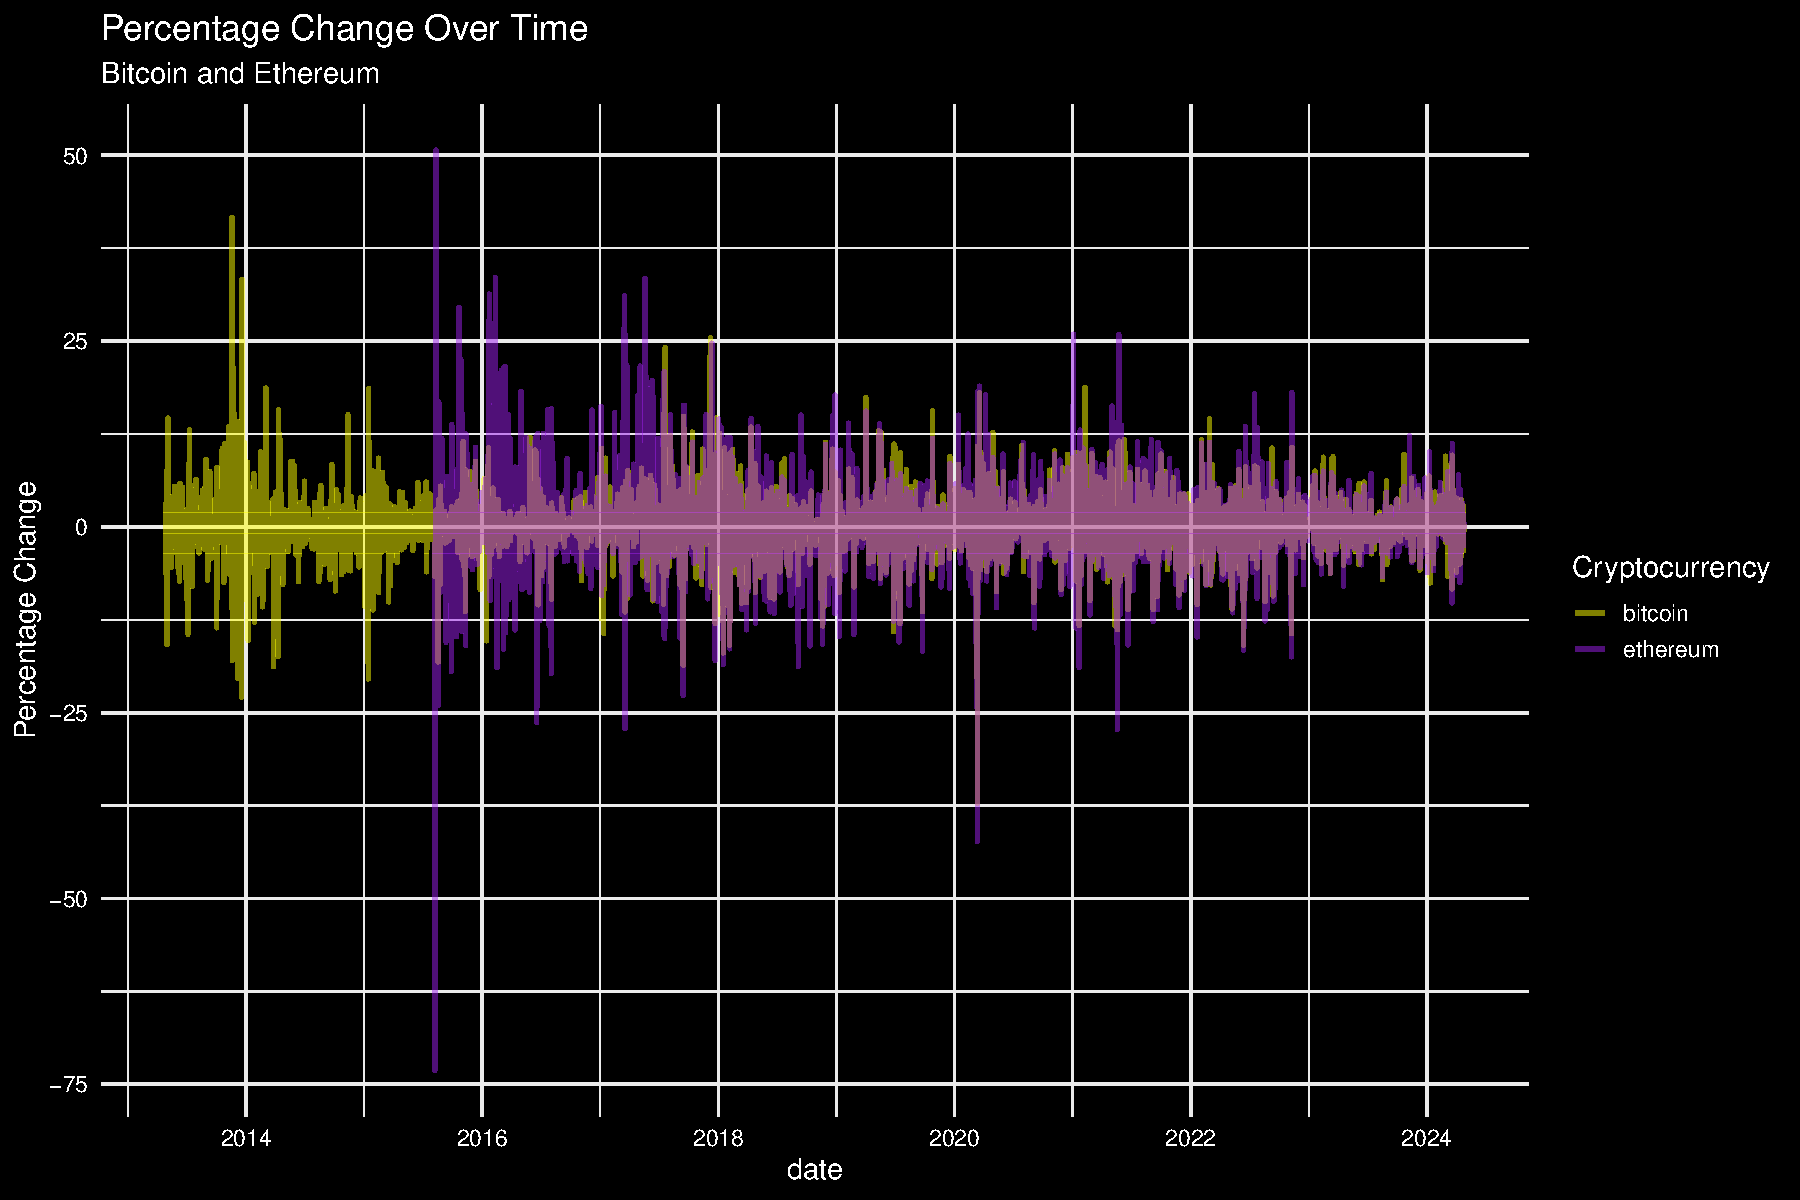
\includegraphics{Crypto_ETL_files/figure-latex/Plot mom qoq 13151-1.pdf}

This plot visualizes the percentage change in market prices for Bitcoin
and Ethereum from 2014 through 2024. The data suggests significant
volatility in both cryptocurrencies, with Ethereum showing a tighter
range of fluctuations in recent years compared to Bitcoin. This analysis
is crucial for strategic investment decisions and risk assessment in the
crypto market.

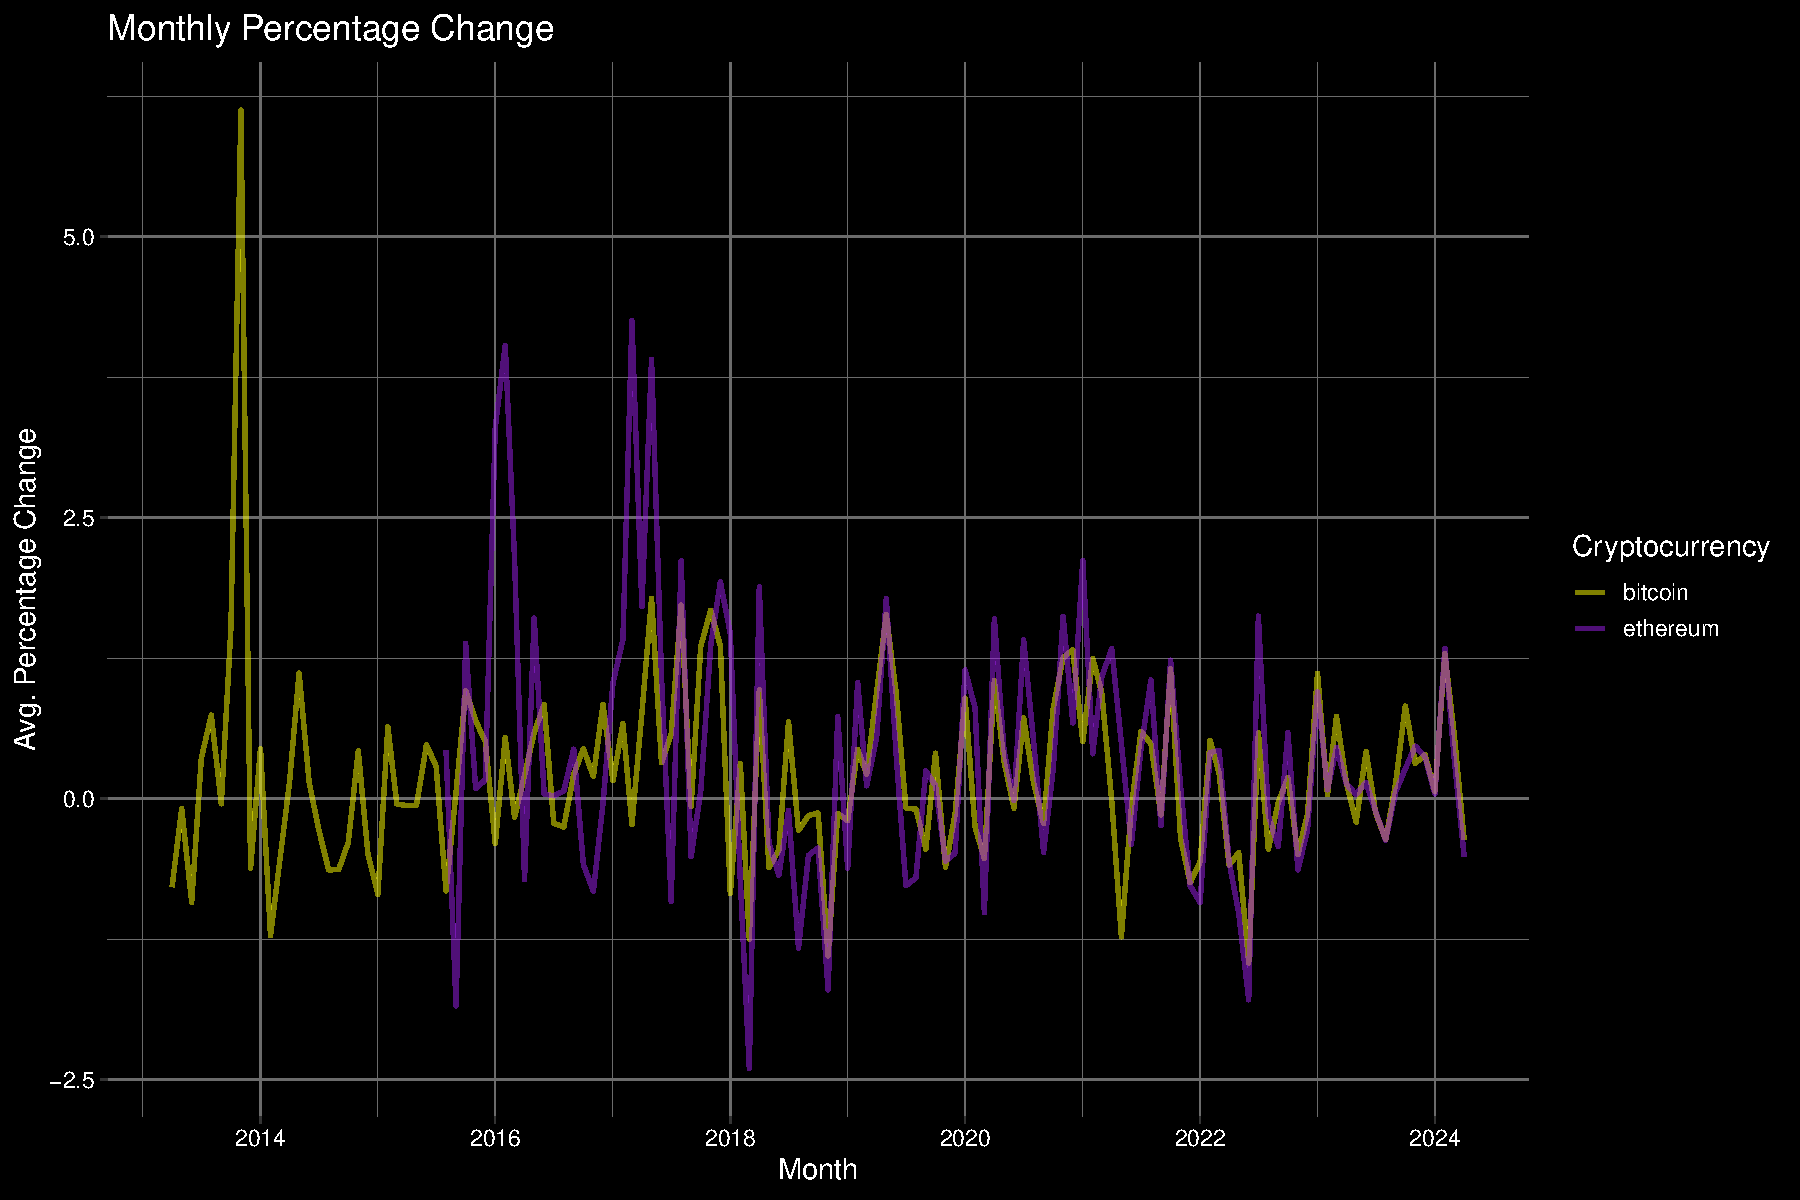
\includegraphics{Crypto_ETL_files/figure-latex/Plot mom qoq 35156153-1.pdf}

This plot displays monthly percentage changes for Bitcoin and Ethereum,
highlighting their historical performance variability. Bitcoin shows
early spikes, whereas Ethereum demonstrates increased volatility around
2016-2018. Investors should consider these trends for potential hedging
strategies and diversifying investment portfolios in the volatile
cryptocurrency market.

\begin{Shaded}
\begin{Highlighting}[]
\CommentTok{\# Aggregate data by quarter}
\NormalTok{df\_pa\_quarter }\OtherTok{\textless{}{-}}\NormalTok{ df\_pa\_filtered }\SpecialCharTok{\%\textgreater{}\%}
  \FunctionTok{mutate}\NormalTok{(}\AttributeTok{Quarter =} \FunctionTok{floor\_date}\NormalTok{(date, }\StringTok{"quarter"}\NormalTok{)) }\SpecialCharTok{\%\textgreater{}\%}
  \FunctionTok{group\_by}\NormalTok{(slug, Quarter) }\SpecialCharTok{\%\textgreater{}\%}
  \FunctionTok{summarize}\NormalTok{(}\AttributeTok{pct\_change =} \FunctionTok{mean}\NormalTok{(pct\_change, }\AttributeTok{na.rm =} \ConstantTok{TRUE}\NormalTok{), }\AttributeTok{.groups =} \StringTok{\textquotesingle{}drop\textquotesingle{}}\NormalTok{)}
\end{Highlighting}
\end{Shaded}

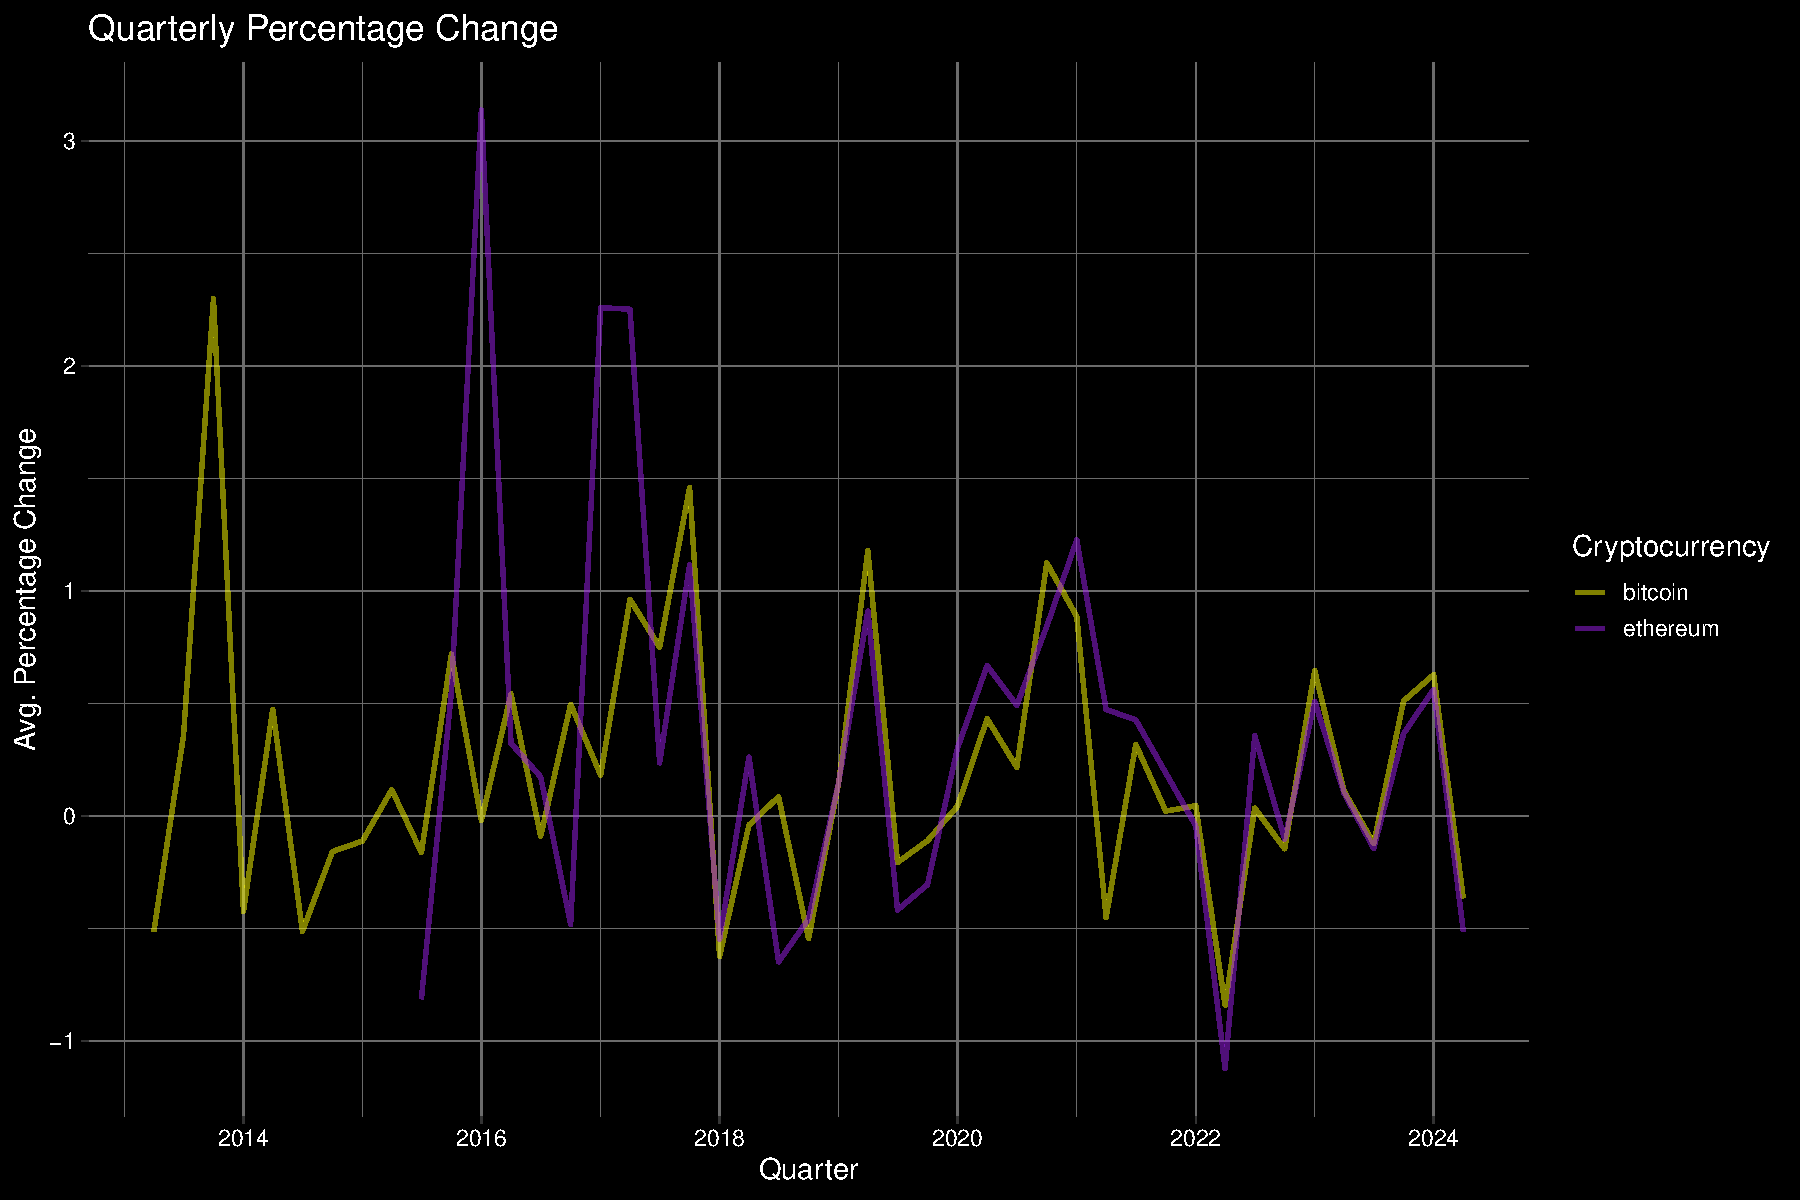
\includegraphics{Crypto_ETL_files/figure-latex/Plot mom qoq-1.pdf}

This chart illustrates the quarterly percentage changes for Bitcoin and
Ethereum. The data indicates fluctuating but generally moderating
volatility over time, crucial for strategizing long-term investment
approaches and risk management in portfolio diversification within the
evolving cryptocurrency market.

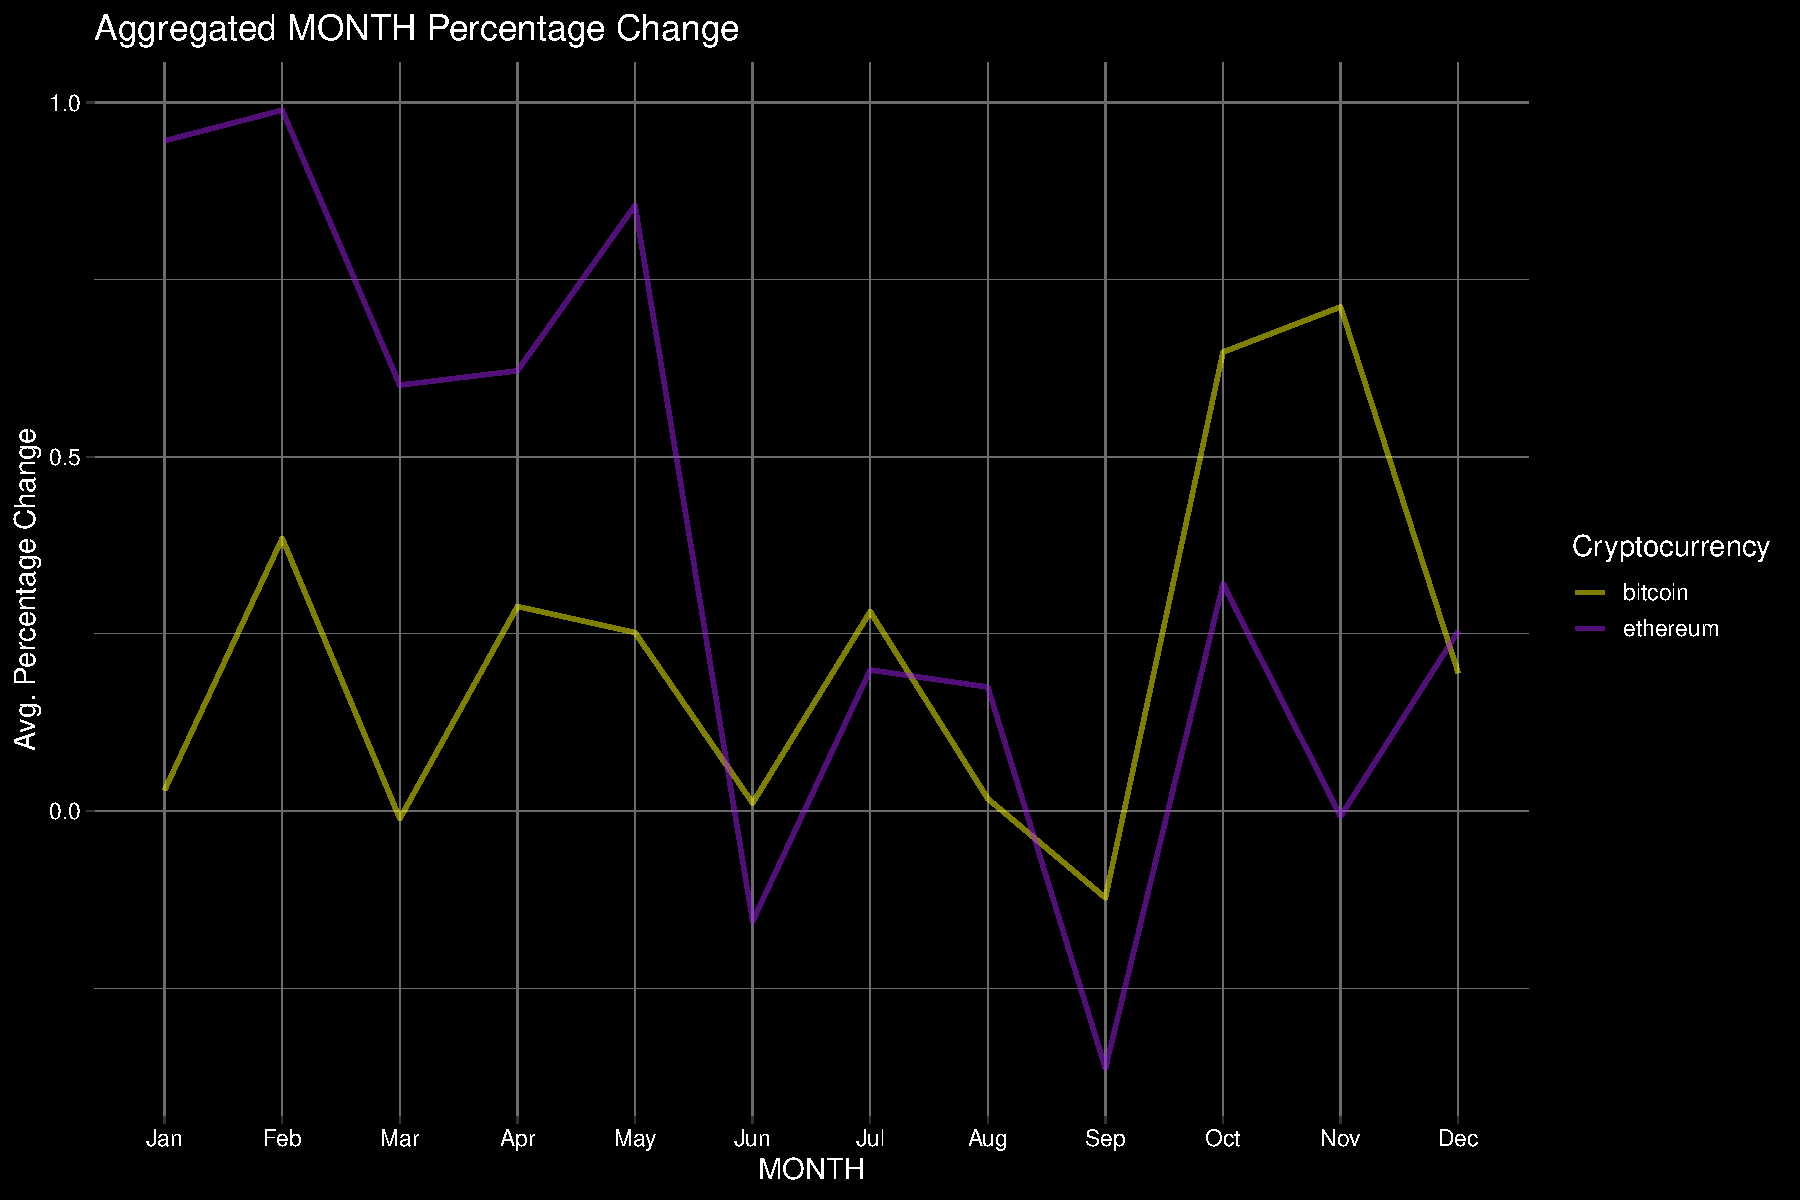
\includegraphics{Crypto_ETL_files/figure-latex/agg plot mom dod qoq code 1-1.pdf}

This chart tracks the aggregated monthly percentage changes in Bitcoin
and Ethereum. The patterns highlight seasonality and monthly performance
trends, essential for crafting targeted investment strategies and
optimizing entry and exit points in the cryptocurrency market.

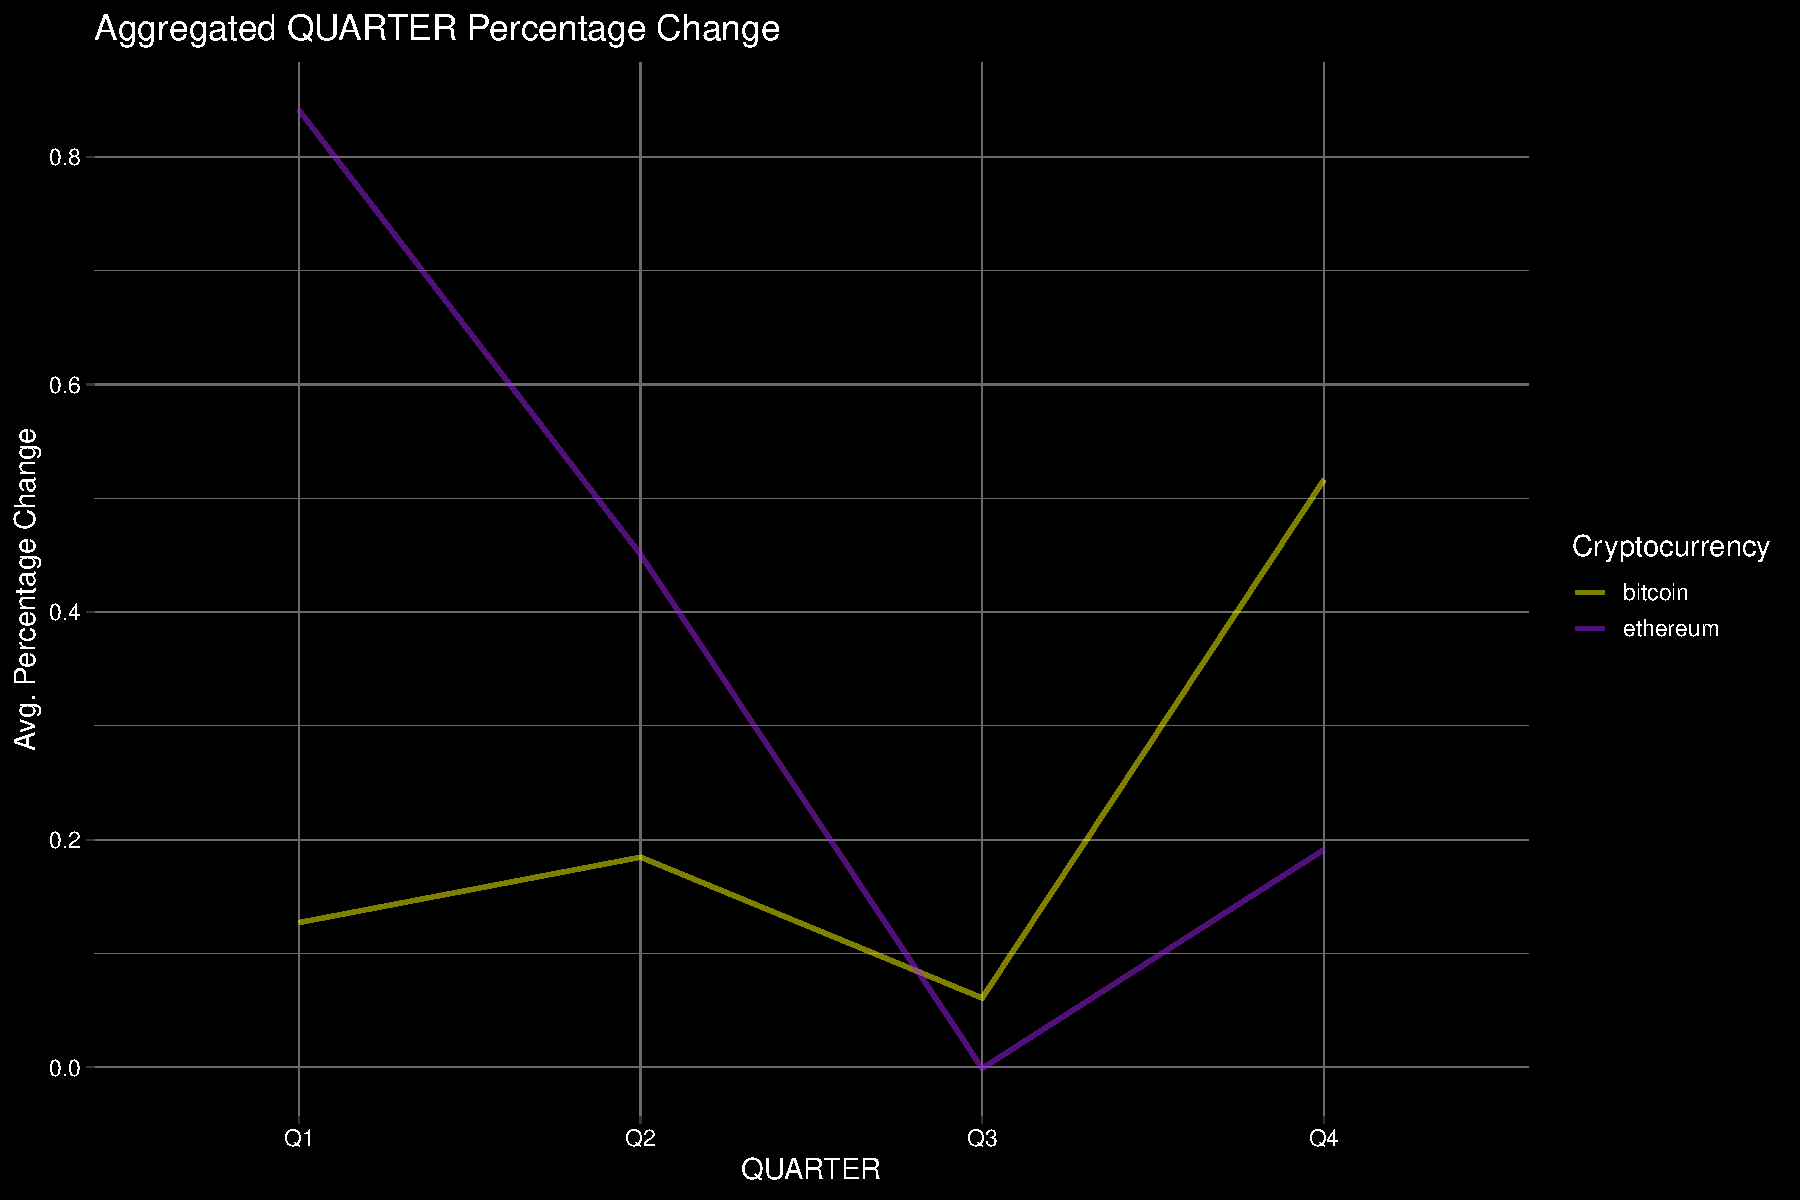
\includegraphics{Crypto_ETL_files/figure-latex/agg plot mom dod qoq code 2 -1.pdf}
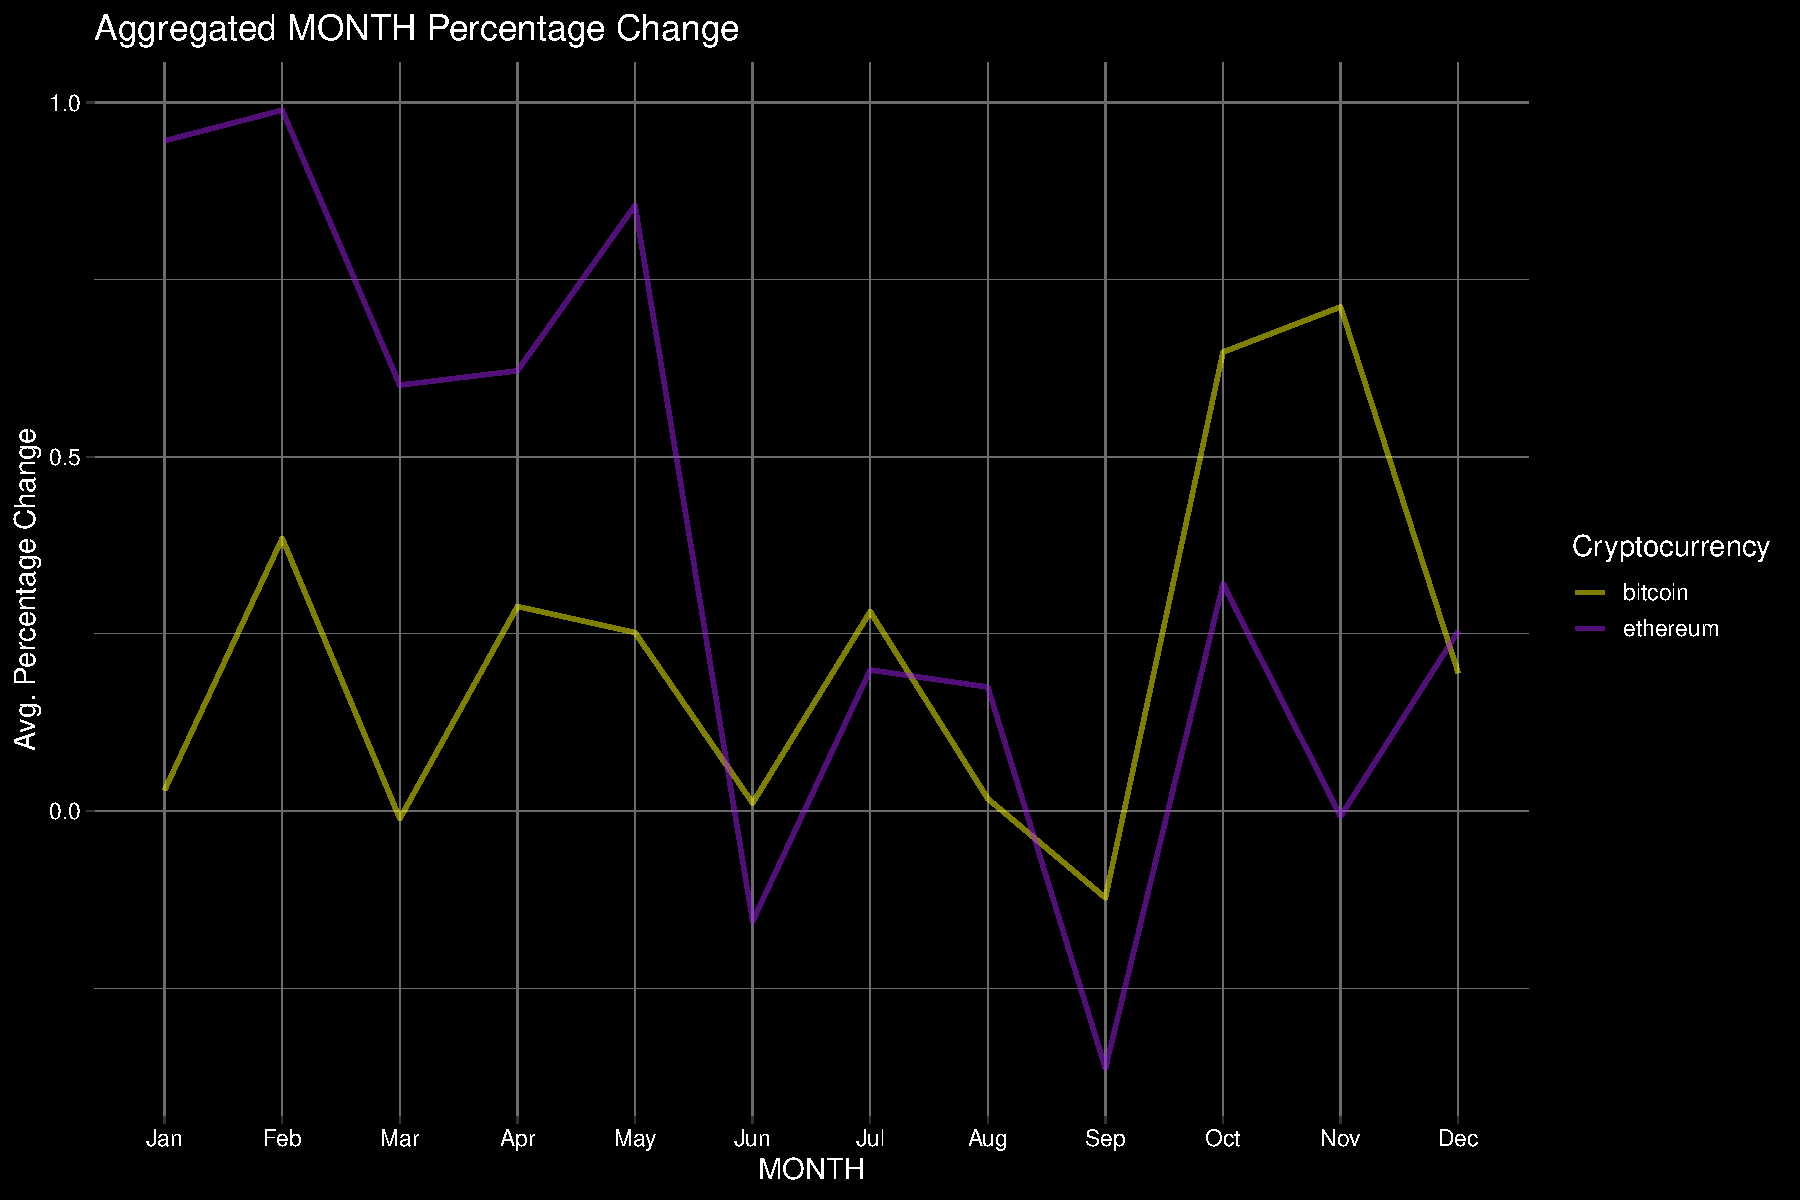
\includegraphics{Crypto_ETL_files/figure-latex/agg plot mom dod qoq code 2 -2.pdf}
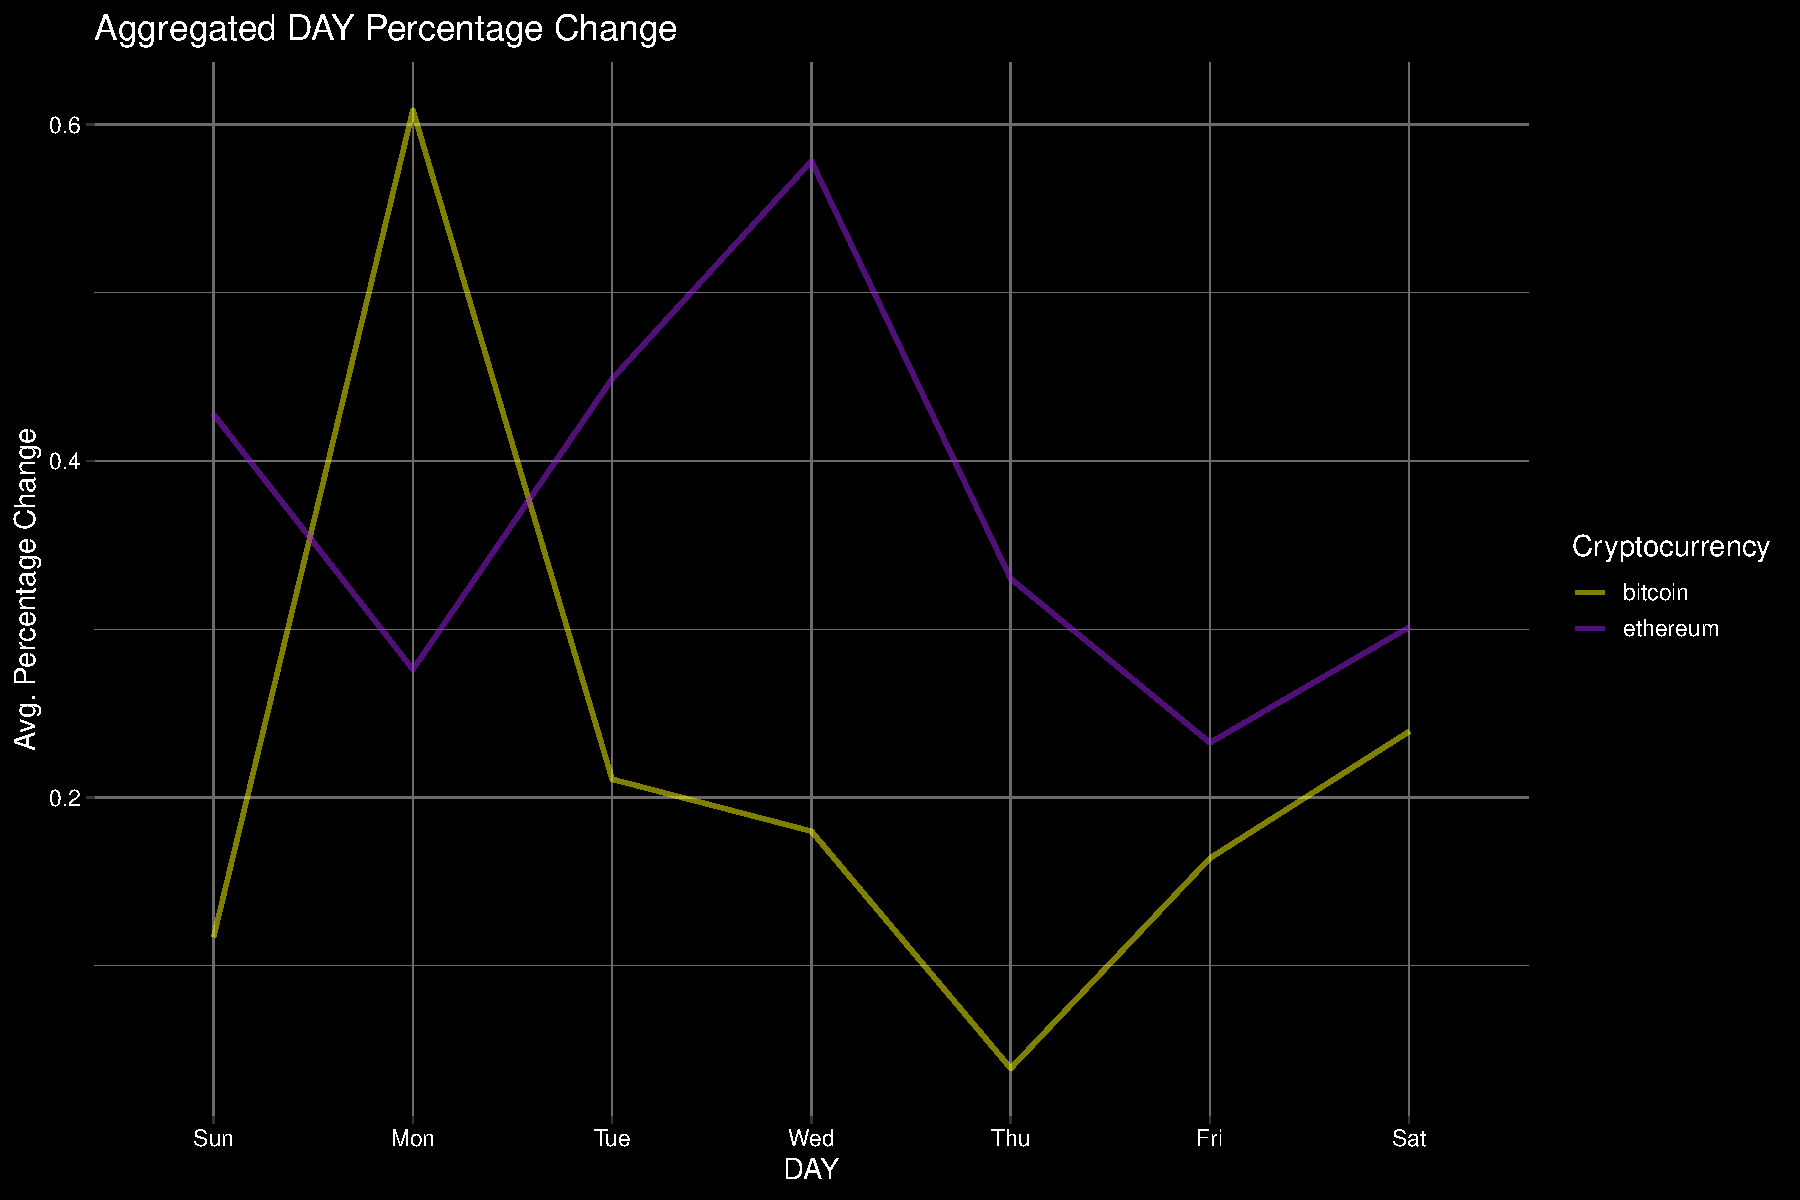
\includegraphics{Crypto_ETL_files/figure-latex/agg plot mom dod qoq code 2 -3.pdf}

\hypertarget{key-observations}{%
\subsection{Key Observations}\label{key-observations}}

\textbf{Midweek Volatility:} Significant spikes in volatility observed
midweek for both cryptocurrencies. Ethereum shows a pronounced increase
on Wednesdays, while Bitcoin peaks on Tuesdays. Suggests increased
trading activity and market-moving events during midweek.

\textbf{Weekend Patterns:} Reduced volatility during weekends,
especially on Sundays. Indicates lower trading activity as markets wind
down and prepare for the upcoming week.

\textbf{Quarterly Trends:} Marked volatility within each quarter with a
notable sharp recovery in Q3. Points to cyclical market sentiment and
macroeconomic influences crucial for timing investment decisions.

\textbf{Monthly Analysis:} Detailed granularity reveals distinct
patterns and seasonality. Both cryptocurrencies show similar trends with
significant gains followed by corrections, especially noticeable around
mid-year and year-end.

\hypertarget{investment-considerations}{%
\subsubsection{Investment
Considerations}\label{investment-considerations}}

\textbf{Risk Management:} By understanding observed patterns, investors
can better anticipate periods of high volatility and adjust their
portfolio exposures to mitigate risks.

\textbf{Strategic Entry and Exit Points:} Data suggests optimal
investment windows, particularly investing at the start of a quarter
post-downturn to capitalize on expected recoveries.

\textbf{Diversification}: Differences in volatility profiles between
Bitcoin and Ethereum suggest opportunities for diversification to
stabilize returns.

\hypertarget{investment-strategy-considerations}{%
\subsubsection{Investment Strategy
Considerations}\label{investment-strategy-considerations}}

\textbf{Day Trading Opportunities:} Heightened midweek volatility offers
potential for day trading, especially from Tuesday to Thursday,
providing opportunities to take early week positions and potentially
exit before the weekend.

\textbf{Risk Management:} Daily market fluctuations necessitate tailored
risk management strategies, including the use of stop-loss orders to
manage potential price movements effectively.

\textbf{Weekend Strategy:} Lower trading activity on weekends allows for
strategic time for portfolio assessment and preparation for the
forthcoming week.

\hypertarget{conclusion}{%
\subsubsection{Conclusion}\label{conclusion}}

\begin{verbatim}
This analysis highlights the importance of understanding market dynamics on daily, monthly, and quarterly bases to form a robust trading and investment strategy. By leveraging these insights, investors and traders can optimize their approaches to maximize returns and minimize risks in the volatile cryptocurrency market, enhancing overall portfolio performance.
\end{verbatim}

\begin{Shaded}
\begin{Highlighting}[]
\FunctionTok{library}\NormalTok{(readxl)}
\NormalTok{key }\OtherTok{\textless{}{-}} \FunctionTok{read\_excel}\NormalTok{(}\StringTok{"\textasciitilde{}/GitHub/CryptoDataFetcher/CryptoDataFetcher2.0/DATA/Keys/MasterDataKey.xlsx"}\NormalTok{)}
\end{Highlighting}
\end{Shaded}

\begin{Shaded}
\begin{Highlighting}[]
\CommentTok{\# Merging the \textquotesingle{}rank\textquotesingle{} column from \textquotesingle{}key\textquotesingle{} into \textquotesingle{}df\textquotesingle{} using \textquotesingle{}id\textquotesingle{} as the key}
\NormalTok{df }\OtherTok{\textless{}{-}}\NormalTok{ df }\SpecialCharTok{\%\textgreater{}\%}
  \FunctionTok{left\_join}\NormalTok{(key }\SpecialCharTok{\%\textgreater{}\%} \FunctionTok{select}\NormalTok{(id, rank), }\AttributeTok{by =} \StringTok{"id"}\NormalTok{)}
\end{Highlighting}
\end{Shaded}

\hypertarget{removing-na-and-inf-values-from-dataset}{%
\paragraph{Removing NA and Inf Values from
Dataset}\label{removing-na-and-inf-values-from-dataset}}

\begin{Shaded}
\begin{Highlighting}[]
\CommentTok{\# Calculate the logarithmic ret, grouped by symbol if necessary for other analyses}
\NormalTok{df\_selected }\OtherTok{\textless{}{-}}\NormalTok{ df\_selected }\SpecialCharTok{\%\textgreater{}\%}
  \FunctionTok{group\_by}\NormalTok{(symbol) }\SpecialCharTok{\%\textgreater{}\%}
  \FunctionTok{mutate}\NormalTok{(}\AttributeTok{log\_ret =} \FunctionTok{log}\NormalTok{(close }\SpecialCharTok{/}\NormalTok{ open)) }\SpecialCharTok{\%\textgreater{}\%}  \CommentTok{\# Calculate log ret as log(close/open)}
  \FunctionTok{ungroup}\NormalTok{()  }\CommentTok{\# optional: ungroup after the mutation if no further grouped operations}

\CommentTok{\# Assuming df\_selected already includes the \textquotesingle{}log\_ret\textquotesingle{} calculations}
\NormalTok{df\_selected }\OtherTok{\textless{}{-}}\NormalTok{ df\_selected }\SpecialCharTok{\%\textgreater{}\%}
  \FunctionTok{group\_by}\NormalTok{(symbol) }\SpecialCharTok{\%\textgreater{}\%}
  \FunctionTok{arrange}\NormalTok{(date) }\SpecialCharTok{\%\textgreater{}\%}  \CommentTok{\# Ensure the data is sorted by date}
  \FunctionTok{mutate}\NormalTok{(}
    \AttributeTok{cum\_log\_ret =} \FunctionTok{cumsum}\NormalTok{(log\_ret)  }\CommentTok{\# Calculate cumulative logarithmic ret}
\NormalTok{  ) }\SpecialCharTok{\%\textgreater{}\%}
  \FunctionTok{ungroup}\NormalTok{()  }\CommentTok{\# Optional: ungroup if no further grouped operations are needed}

\CommentTok{\# Optionally, round cum\_ret to 2 decimal places if needed for consistency}
\NormalTok{df\_selected}\SpecialCharTok{$}\NormalTok{log\_ret }\OtherTok{\textless{}{-}} \FunctionTok{round}\NormalTok{(df\_selected}\SpecialCharTok{$}\NormalTok{log\_ret, }\DecValTok{2}\NormalTok{)}
\CommentTok{\# Optionally, round cum\_ret to 2 decimal places if needed for consistency}
\NormalTok{df\_selected}\SpecialCharTok{$}\NormalTok{cum\_log\_ret }\OtherTok{\textless{}{-}} \FunctionTok{round}\NormalTok{(df\_selected}\SpecialCharTok{$}\NormalTok{cum\_log\_ret, }\DecValTok{2}\NormalTok{)}

\CommentTok{\# Print the updated data frame to verify the results}
\FunctionTok{print}\NormalTok{(df\_selected)}
\end{Highlighting}
\end{Shaded}

\begin{verbatim}
## # A tibble: 821,090 x 11
##    slug   symbol date         open  close market_cap  rank   ret cum_ret log_ret
##    <chr>  <chr>  <date>      <dbl>  <dbl>      <dbl> <dbl> <dbl>   <dbl>   <dbl>
##  1 bitco~ BTC    2013-04-28 137.   128.       1.42e9     1 -0.06   -0.06   -0.07
##  2 bitco~ BTC    2013-04-29 134.   145.       1.60e9     1  0.08    0.02    0.07
##  3 litec~ LTC    2013-04-29   4.37   4.38     7.54e7    19  0       0       0   
##  4 bitco~ BTC    2013-04-30 144    139        1.54e9     1 -0.03   -0.02   -0.04
##  5 litec~ LTC    2013-04-30   4.4    4.3      7.40e7    19 -0.02   -0.02   -0.02
##  6 bitco~ BTC    2013-05-01 139    117.       1.30e9     1 -0.16   -0.17   -0.17
##  7 litec~ LTC    2013-05-01   4.29   3.8      6.56e7    19 -0.11   -0.13   -0.12
##  8 bitco~ BTC    2013-05-02 116.   105.       1.17e9     1 -0.1    -0.26   -0.1 
##  9 litec~ LTC    2013-05-02   3.78   3.37     5.83e7    19 -0.11   -0.22   -0.11
## 10 bitco~ BTC    2013-05-03 106.    97.8      1.09e9     1 -0.08   -0.32   -0.08
## # i 821,080 more rows
## # i 1 more variable: cum_log_ret <dbl>
\end{verbatim}

\begin{Shaded}
\begin{Highlighting}[]
\CommentTok{\#write.csv(df\_selected, "Crypto\_Hist\_LogRt.csv", row.names = FALSE)}
\end{Highlighting}
\end{Shaded}

\begin{Shaded}
\begin{Highlighting}[]
\CommentTok{\#for later when we have all the other data pct change as well as log date structureed like MoM or DoD}
\end{Highlighting}
\end{Shaded}

\hypertarget{halving-dates-pre-n-post-halving-dates}{%
\section{Halving dates pre n post halving
dates}\label{halving-dates-pre-n-post-halving-dates}}

\emph{**Analysis Objectives and Methods**: We've focused on extracting
and analyzing data from significant periods around each Bitcoin halving
event, which occurs approximately every four years, reducing the reward
for mining new blocks by half. This reduction potentially influences
Bitcoin's price due to decreased supply flow. By comparing the market
dynamics pre and post halving, we seek to identify patterns or trends
that could inform investment strategies and economic forecasts related
to Bitcoin.}

\emph{Key Achievements:}

\begin{enumerate}
\def\labelenumi{\arabic{enumi}.}
\item
  \textbf{Trend Identification:} We have identified trends in price
  fluctuations and market cap changes surrounding the halving dates,
  providing insights into the cyclical nature of Bitcoin's market
  valuation.
\item
  \textbf{Comparative Analysis:} By juxtaposing data from different
  halving periods, we've been able to observe the evolution in market
  reactions over multiple cycles, discerning if reactions have become
  more pronounced or stabilized as the market matures.
\item
  \textbf{Predictive Insights:} Understanding past patterns allows us to
  forecast potential future price movements around subsequent halvings,
  offering valuable information for investors and market analysts.
\end{enumerate}

\textbf{Importance of the Analysis:} This analysis is crucial for
several reasons:

\begin{itemize}
\item
  \textbf{Investor Guidance:} It helps investors understand potential
  price movements and manage risks associated with Bitcoin investments
  around halving events.
\item
  \textbf{Economic Implications:} It provides insights into how major
  supply changes in a dominant cryptocurrency can affect broader
  financial markets.
\item
  \textbf{Enhanced Understanding of Market Dynamics:} It contributes to
  the academic and practical understanding of cryptocurrency economics,
  particularly how supply constraints can impact asset prices.
\end{itemize}

\begin{Shaded}
\begin{Highlighting}[]
\CommentTok{\# Update the last entry in the \textquotesingle{}Halving\textquotesingle{} column}
\NormalTok{df\_periods[}\FunctionTok{nrow}\NormalTok{(df\_periods), }\StringTok{\textquotesingle{}Halving\textquotesingle{}}\NormalTok{] }\OtherTok{\textless{}{-}} \StringTok{\textquotesingle{}2024 Halving\textquotesingle{}}

\CommentTok{\# Check the updated data frame}
\FunctionTok{print}\NormalTok{(df\_periods)}
\end{Highlighting}
\end{Shaded}

\begin{verbatim}
## # A tibble: 16 x 9
##    Halving      Period   Start_Date End_Date    days weeks months quarters years
##    <chr>        <chr>    <date>     <date>     <int> <dbl>  <dbl>    <dbl> <dbl>
##  1 2012 Halving Pre-Bull 2012-03-01 2012-10-31   244    35      8        3     1
##  2 2014 Halving Halving~ 2012-11-01 2012-11-01     0     0      0        0     0
##  3 2014 Halving Bull Run 2012-11-02 2014-07-08   613    88     20        7     2
##  4 2014 Halving Crypto ~ 2014-07-09 2015-09-01   419    60     14        5     1
##  5 2016 Halving Pre-Bull 2015-09-02 2016-07-08   310    44     10        3     1
##  6 2016 Halving Halving~ 2016-07-09 2016-07-09     0     0      0        0     0
##  7 2016 Halving Bull Run 2016-07-10 2017-12-31   539    77     18        6     1
##  8 2016 Halving Crypto ~ 2017-01-01 2019-01-01   730   104     24        8     2
##  9 2020 Halving Pre-Bull 2019-01-02 2020-05-11   495    71     16        5     1
## 10 2020 Halving Halving~ 2020-05-12 2020-05-12     0     0      0        0     0
## 11 2020 Halving Bull Run 2020-05-13 2021-03-01   292    42     10        3     1
## 12 2020 Halving Crypto ~ 2021-03-02 2021-07-01   121    17      4        1     0
## 13 2020 Halving Bull Run 2021-07-02 2021-11-01   122    17      4        1     0
## 14 2020 Halving Crypto ~ 2021-11-02 2022-12-01   394    56     13        4     1
## 15 2024 Halving Pre-Bull 2022-12-02 2024-04-19   504    72     17        6     1
## 16 2024 Halving Halving~ 2024-04-20 2024-04-20     0     0      0        0     0
\end{verbatim}

\begin{Shaded}
\begin{Highlighting}[]
\NormalTok{HalvingDatesKey}\OtherTok{\textless{}{-}}\NormalTok{df\_periods}
\FunctionTok{write.csv}\NormalTok{(HalvingDatesKey, }\StringTok{"HalvingDataKey.csv"}\NormalTok{, }\AttributeTok{row.names =} \ConstantTok{FALSE}\NormalTok{)}
\end{Highlighting}
\end{Shaded}

\begin{Shaded}
\begin{Highlighting}[]
\CommentTok{\# Assuming the date format needs to be converted in both data frames}
\NormalTok{MasterCrypto}\SpecialCharTok{$}\NormalTok{date }\OtherTok{\textless{}{-}} \FunctionTok{as.Date}\NormalTok{(MasterCrypto}\SpecialCharTok{$}\NormalTok{date, }\AttributeTok{format=}\StringTok{"\%Y{-}\%m{-}\%d"}\NormalTok{)}

\CommentTok{\# Assuming df\_periods already loaded from earlier steps, format its dates if not done already}
\NormalTok{df\_periods}\SpecialCharTok{$}\NormalTok{Start\_Date }\OtherTok{\textless{}{-}} \FunctionTok{as.Date}\NormalTok{(df\_periods}\SpecialCharTok{$}\NormalTok{Start\_Date, }\AttributeTok{format=}\StringTok{"\%Y{-}\%m{-}\%d"}\NormalTok{)}
\NormalTok{df\_periods}\SpecialCharTok{$}\NormalTok{End\_Date }\OtherTok{\textless{}{-}} \FunctionTok{as.Date}\NormalTok{(df\_periods}\SpecialCharTok{$}\NormalTok{End\_Date, }\AttributeTok{format=}\StringTok{"\%Y{-}\%m{-}\%d"}\NormalTok{)}
\end{Highlighting}
\end{Shaded}

\begin{Shaded}
\begin{Highlighting}[]
\ControlFlowTok{if}\NormalTok{ (}\SpecialCharTok{!}\FunctionTok{require}\NormalTok{(}\StringTok{"fuzzyjoin"}\NormalTok{)) }\FunctionTok{install.packages}\NormalTok{(}\StringTok{"fuzzyjoin"}\NormalTok{)}
\FunctionTok{library}\NormalTok{(fuzzyjoin)}

\CommentTok{\# Perform a fuzzy join based on date ranges}
\NormalTok{df\_merged }\OtherTok{\textless{}{-}} \FunctionTok{fuzzy\_left\_join}\NormalTok{(MasterCrypto, df\_periods,}
                             \AttributeTok{by =} \FunctionTok{c}\NormalTok{(}\StringTok{"date"} \OtherTok{=} \StringTok{"Start\_Date"}\NormalTok{, }\StringTok{"date"} \OtherTok{=} \StringTok{"End\_Date"}\NormalTok{),}
                             \AttributeTok{match\_fun =} \FunctionTok{list}\NormalTok{(}\StringTok{\textasciigrave{}}\AttributeTok{\textgreater{}=}\StringTok{\textasciigrave{}}\NormalTok{, }\StringTok{\textasciigrave{}}\AttributeTok{\textless{}=}\StringTok{\textasciigrave{}}\NormalTok{))}

\CommentTok{\# After the join, select all columns from MasterCrypto and the Code column from df\_periods}
\NormalTok{df\_merged }\OtherTok{\textless{}{-}}\NormalTok{ df\_merged }\SpecialCharTok{\%\textgreater{}\%}
  \FunctionTok{select}\NormalTok{(}\FunctionTok{all\_of}\NormalTok{(}\FunctionTok{names}\NormalTok{(MasterCrypto)), }\AttributeTok{Code =}\NormalTok{ Code)}

\NormalTok{Crypto\_Hist\_Ret\_Log\_Rank\_Code }\OtherTok{\textless{}{-}}\NormalTok{ df\_merged}

\CommentTok{\#write.csv(Crypto\_Hist\_Ret\_Log\_Rank\_Code, "Crypto\_Hist\_Ret\_Log\_Rank\_Code.csv", row.names = FALSE)}
\end{Highlighting}
\end{Shaded}

\hypertarget{halving-analysis}{%
\subsection{Halving Analysis}\label{halving-analysis}}

\begin{Shaded}
\begin{Highlighting}[]
\NormalTok{halving\_2016 }\OtherTok{\textless{}{-}}\NormalTok{ df\_merged }\SpecialCharTok{\%\textgreater{}\%} \FunctionTok{filter}\NormalTok{(date }\SpecialCharTok{==} \FunctionTok{as.Date}\NormalTok{(}\StringTok{"2016{-}07{-}09"}\NormalTok{))}
\NormalTok{halving\_2020 }\OtherTok{\textless{}{-}}\NormalTok{ df\_merged }\SpecialCharTok{\%\textgreater{}\%} \FunctionTok{filter}\NormalTok{(date }\SpecialCharTok{==} \FunctionTok{as.Date}\NormalTok{(}\StringTok{"2020{-}05{-}12"}\NormalTok{))}
\NormalTok{halving\_2024 }\OtherTok{\textless{}{-}}\NormalTok{ df\_merged }\SpecialCharTok{\%\textgreater{}\%} \FunctionTok{filter}\NormalTok{(date }\SpecialCharTok{==} \FunctionTok{as.Date}\NormalTok{(}\StringTok{"2024{-}04{-}20"}\NormalTok{))}
\end{Highlighting}
\end{Shaded}

\begin{Shaded}
\begin{Highlighting}[]
\FunctionTok{library}\NormalTok{(dplyr)}
\FunctionTok{library}\NormalTok{(ggplot2)}
\FunctionTok{library}\NormalTok{(lubridate)}

\CommentTok{\# Combining and creating a unified data frame with 2016, 2020, and 2024 data}
\NormalTok{combined\_halving\_data }\OtherTok{\textless{}{-}} \FunctionTok{bind\_rows}\NormalTok{(}
  \FunctionTok{list}\NormalTok{(halving\_2016, halving\_2020, halving\_2024),}
  \AttributeTok{.id =} \StringTok{"Halving\_Year"}
\NormalTok{) }\SpecialCharTok{\%\textgreater{}\%}
  \FunctionTok{mutate}\NormalTok{(}\AttributeTok{Halving\_Year =} \FunctionTok{case\_when}\NormalTok{(}
\NormalTok{    Halving\_Year }\SpecialCharTok{==} \StringTok{"1"} \SpecialCharTok{\textasciitilde{}} \StringTok{"2016"}\NormalTok{,}
\NormalTok{    Halving\_Year }\SpecialCharTok{==} \StringTok{"2"} \SpecialCharTok{\textasciitilde{}} \StringTok{"2020"}\NormalTok{,}
\NormalTok{    Halving\_Year }\SpecialCharTok{==} \StringTok{"3"} \SpecialCharTok{\textasciitilde{}} \StringTok{"2024"}
\NormalTok{  ))}

\CommentTok{\# Get top 25 for each year using group\_by and slice\_max}
\NormalTok{top\_halvings }\OtherTok{\textless{}{-}}\NormalTok{ combined\_halving\_data }\SpecialCharTok{\%\textgreater{}\%}
  \FunctionTok{group\_by}\NormalTok{(Halving\_Year) }\SpecialCharTok{\%\textgreater{}\%}
  \FunctionTok{slice\_max}\NormalTok{(}\AttributeTok{order\_by =}\NormalTok{ market\_cap, }\AttributeTok{n =} \DecValTok{25}\NormalTok{) }\SpecialCharTok{\%\textgreater{}\%}
  \FunctionTok{ungroup}\NormalTok{()  }\CommentTok{\# Ungroup to remove grouping before plotting}

\CommentTok{\# Plotting the data with legend and corrected title and axis rotations}
\FunctionTok{ggplot}\NormalTok{(top\_halvings, }\FunctionTok{aes}\NormalTok{(}\AttributeTok{x =} \FunctionTok{reorder}\NormalTok{(symbol, market\_cap), }\AttributeTok{y =}\NormalTok{ market\_cap, }\AttributeTok{fill =}\NormalTok{ Halving\_Year)) }\SpecialCharTok{+}
  \FunctionTok{geom\_col}\NormalTok{(}\AttributeTok{show.legend =} \ConstantTok{TRUE}\NormalTok{, }\AttributeTok{alpha =} \FloatTok{0.5}\NormalTok{) }\SpecialCharTok{+}
  \FunctionTok{labs}\NormalTok{(}
    \AttributeTok{title =} \StringTok{"Top 25 Cryptocurrencies by Market Cap for Selected Halving Years"}\NormalTok{, }
    \AttributeTok{x =} \StringTok{"Cryptocurrency"}\NormalTok{, }
    \AttributeTok{y =} \StringTok{"Market Cap"}\NormalTok{,}
    \AttributeTok{fill =} \StringTok{"Halving Year"}  \CommentTok{\# Legend title}
\NormalTok{  ) }\SpecialCharTok{+}
  \FunctionTok{scale\_y\_log10}\NormalTok{() }\SpecialCharTok{+}  \CommentTok{\# Apply log10 scale to the y{-}axis}
  \FunctionTok{scale\_fill\_manual}\NormalTok{(}\AttributeTok{values =} \FunctionTok{c}\NormalTok{(}\StringTok{"2016"} \OtherTok{=} \StringTok{"green"}\NormalTok{, }\StringTok{"2020"} \OtherTok{=} \StringTok{"blue"}\NormalTok{, }\StringTok{"2024"} \OtherTok{=} \StringTok{"red"}\NormalTok{)) }\SpecialCharTok{+}
  \FunctionTok{theme\_minimal}\NormalTok{() }\SpecialCharTok{+}
  \FunctionTok{theme}\NormalTok{(}
    \AttributeTok{legend.position =} \StringTok{"bottom"}\NormalTok{,}
    \AttributeTok{axis.text.x =} \FunctionTok{element\_text}\NormalTok{(}\AttributeTok{angle =} \DecValTok{45}\NormalTok{, }\AttributeTok{vjust =} \DecValTok{1}\NormalTok{, }\AttributeTok{hjust =} \DecValTok{1}\NormalTok{)  }\CommentTok{\# Tilt x{-}axis labels by 45 degrees}
\NormalTok{  )}
\end{Highlighting}
\end{Shaded}

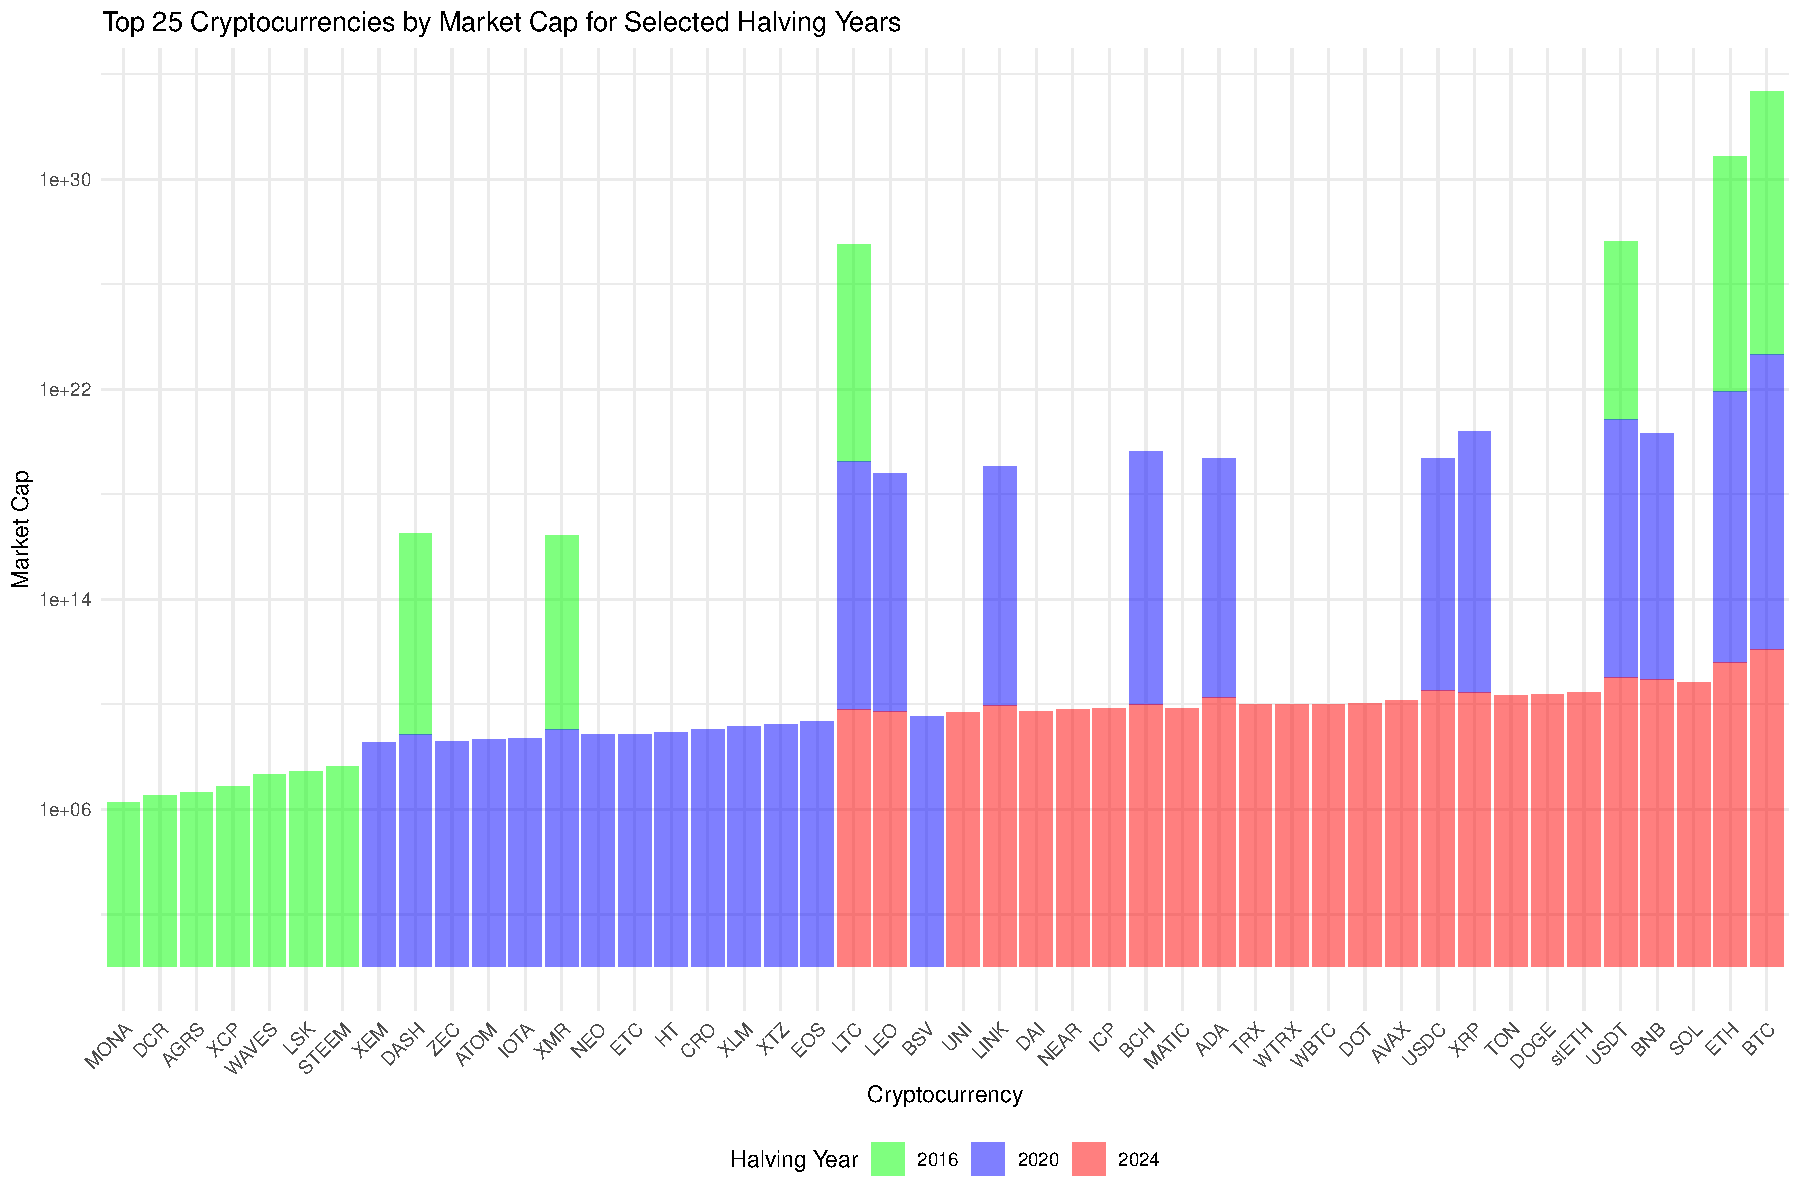
\includegraphics{Crypto_ETL_files/figure-latex/unnamed-chunk-4-1.pdf}

\emph{The bar chart illustrates the market cap of the top 25
cryptocurrencies during Bitcoin halving years (2008, 2012, 2016, and
2024), showcasing distinct patterns:}

\begin{itemize}
\item
  \textbf{Growth Over Time}: The chart shows a clear upward trend in the
  market cap of cryptocurrencies over the selected halving years,
  indicating substantial growth in the crypto market.
\item
  \textbf{Yearly Comparison}: Each halving year, depicted in different
  colors, highlights a significant increase in market cap, with 2024
  showing the most considerable escalation, suggesting increased market
  maturity and investor interest.
\item
  \textbf{Cryptocurrency Diversity}: While some cryptocurrencies
  consistently show growth, others have varying degrees of market cap
  across different years, pointing to shifting investor preferences and
  the dynamic nature of the cryptocurrency market.
\end{itemize}

\begin{verbatim}
## 
## Attaching package: 'plotly'
\end{verbatim}

\begin{verbatim}
## The following object is masked from 'package:ggplot2':
## 
##     last_plot
\end{verbatim}

\begin{verbatim}
## The following object is masked from 'package:stats':
## 
##     filter
\end{verbatim}

\begin{verbatim}
## The following object is masked from 'package:graphics':
## 
##     layout
\end{verbatim}

\begin{verbatim}
## PhantomJS not found. You can install it with webshot::install_phantomjs(). If it is installed, please make sure the phantomjs executable can be found via the PATH variable.
\end{verbatim}

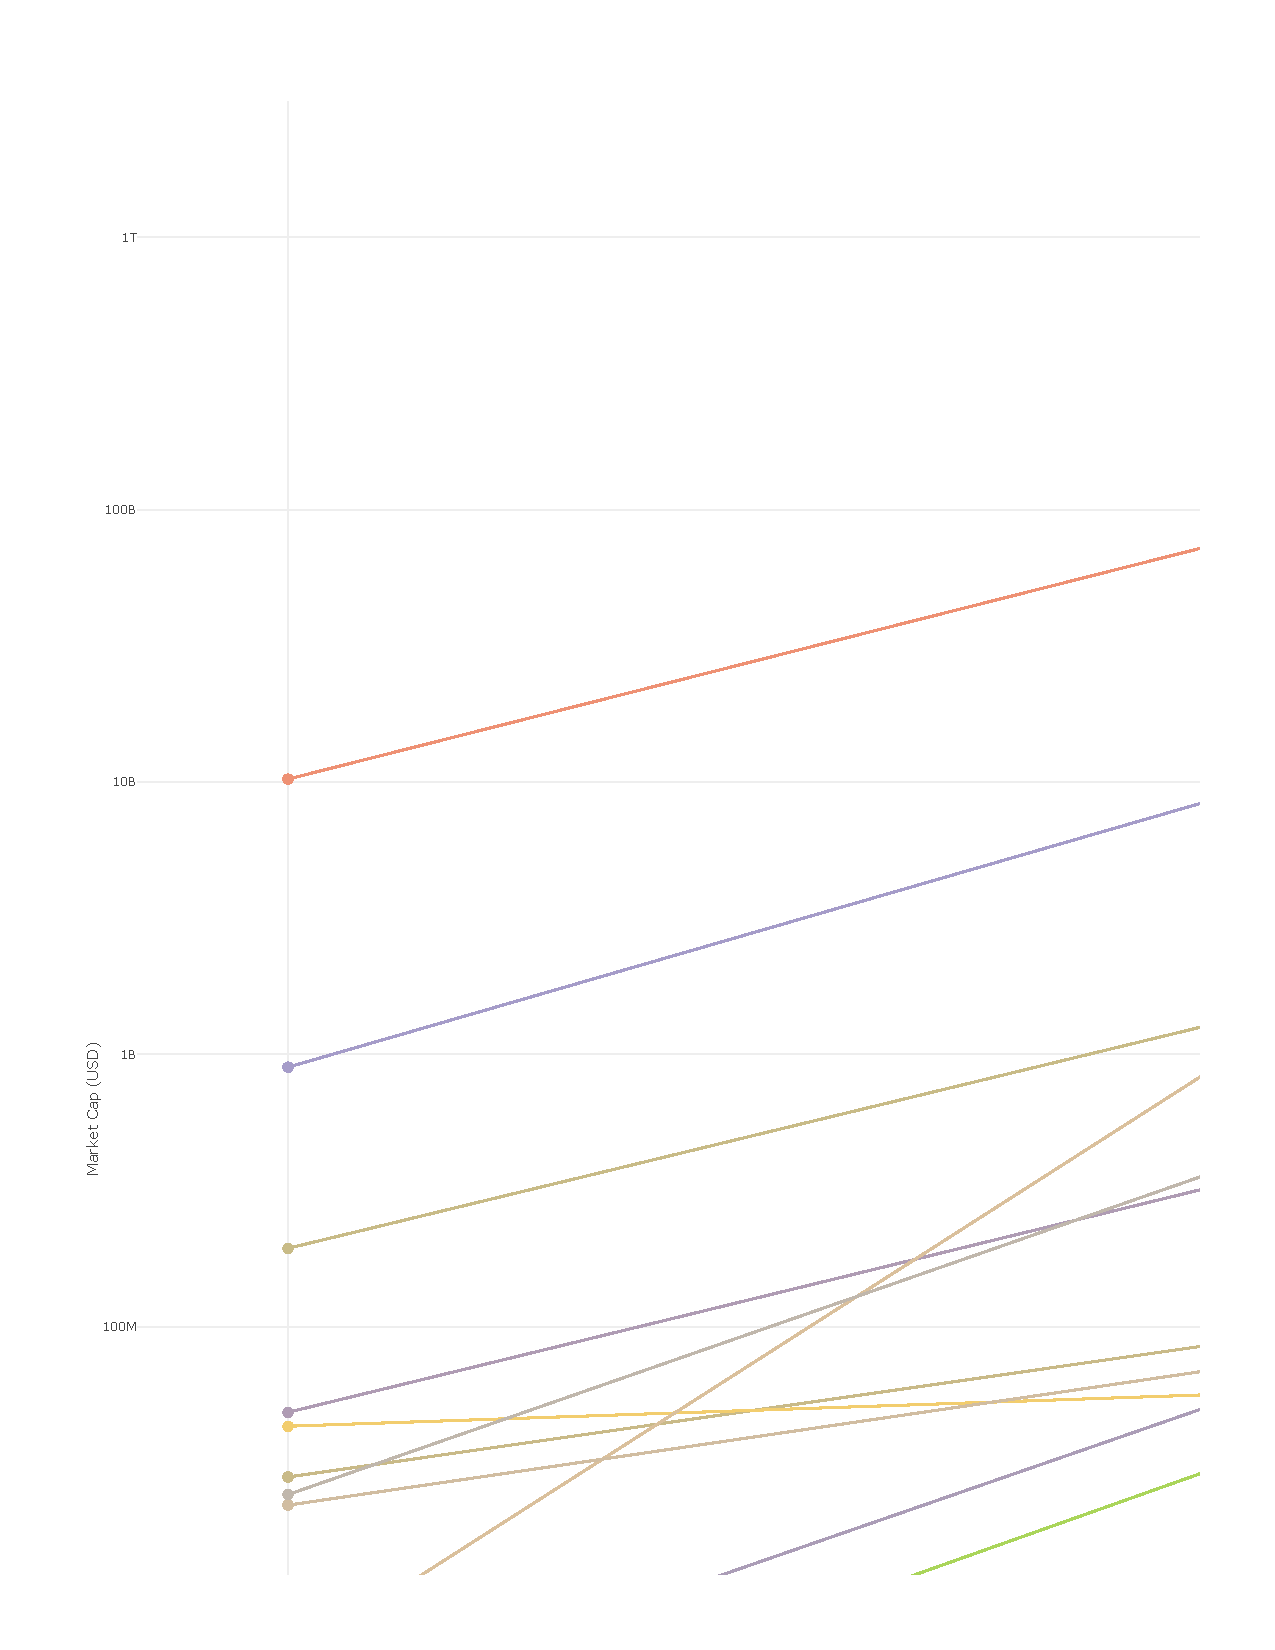
\includegraphics{Crypto_ETL_files/figure-latex/top_crypto_data-1.pdf}
\#\#\#\#\# Impact of Halvings on Market Capitalization: Pre-Halving
Surge: Leading up to the halving events (marked by the vertical lines),
there's often a noticeable increase in market capitalization for many
cryptocurrencies. This trend is driven by anticipation and speculation,
as traders expect the reduced supply of new coins to push prices higher.
Post-Halving Reaction: After the halving, the market reactions can be
mixed. While some cryptocurrencies continue to appreciate due to the
decreased rate of new coin introduction, others may stagnate or decline
as the speculative fervor dies down.

\hypertarget{survival-through-crypto-winters}{%
\subparagraph{Survival Through Crypto
Winters:}\label{survival-through-crypto-winters}}

\begin{verbatim}
    Decline of Many Coins: As visible in your chart, while a few cryptocurrencies sustain growth post-halving, many others experience a sharp decline in market capitalization. This period, often referred to as the “crypto winter,” can be harsh, and many smaller or less established cryptocurrencies might not recover.
\end{verbatim}

\hypertarget{sustainability-of-major-coins-the-major-cryptocurrencies-often-depicted-by-bolder-or-differently-colored-lines-tend-to-show-resilience-and-a-tendency-to-recover-and-grow-in-the-long-term.-this-resilience-is-likely-due-to-stronger-community-support-better-liquidity-and-more-widespread-adoption.}{%
\subparagraph{Sustainability of Major Coins: The major cryptocurrencies
often depicted by bolder or differently colored lines, tend to show
resilience and a tendency to recover and grow in the long term. This
resilience is likely due to stronger community support, better
liquidity, and more widespread
adoption.}\label{sustainability-of-major-coins-the-major-cryptocurrencies-often-depicted-by-bolder-or-differently-colored-lines-tend-to-show-resilience-and-a-tendency-to-recover-and-grow-in-the-long-term.-this-resilience-is-likely-due-to-stronger-community-support-better-liquidity-and-more-widespread-adoption.}}

\hypertarget{importance-of-timely-exits}{%
\subparagraph{Importance of Timely
Exits:}\label{importance-of-timely-exits}}

\begin{verbatim}
    Timing Market Exits: The data underscores the critical nature of timing when investing in cryptocurrencies, especially around such high-impact events as halvings. Investors who exit before the onset of a crypto winter can preserve gains and avoid significant losses.
\end{verbatim}

\hypertarget{strategic-investment-decisions-understanding-the-cyclical-nature-of-cryptocurrencieshighlighted-by-these-halving-eventscan-aid-in-making-informed-decisions-about-when-to-enter-or-exit-positions.-monitoring-not-just-the-halving-dates-but-also-market-sentiment-technological-advancements-and-regulatory-developments-is-crucial.}{%
\subparagraph{Strategic Investment Decisions: Understanding the cyclical
nature of cryptocurrencies---highlighted by these halving events---can
aid in making informed decisions about when to enter or exit positions.
Monitoring not just the halving dates but also market sentiment,
technological advancements, and regulatory developments is
crucial.}\label{strategic-investment-decisions-understanding-the-cyclical-nature-of-cryptocurrencieshighlighted-by-these-halving-eventscan-aid-in-making-informed-decisions-about-when-to-enter-or-exit-positions.-monitoring-not-just-the-halving-dates-but-also-market-sentiment-technological-advancements-and-regulatory-developments-is-crucial.}}

\textbf{\emph{In summary, your chart powerfully illustrates the volatile
nature of the cryptocurrency market, influenced heavily by periodic
halving events. For investors and traders, the key takeaway would be the
importance of strategic entries and exits, recognizing the signs of an
impending downturn, and choosing cryptocurrencies with strong
fundamentals and market support. This approach could mitigate risks
associated with the inevitable fluctuations and downturns
post-halving.}}
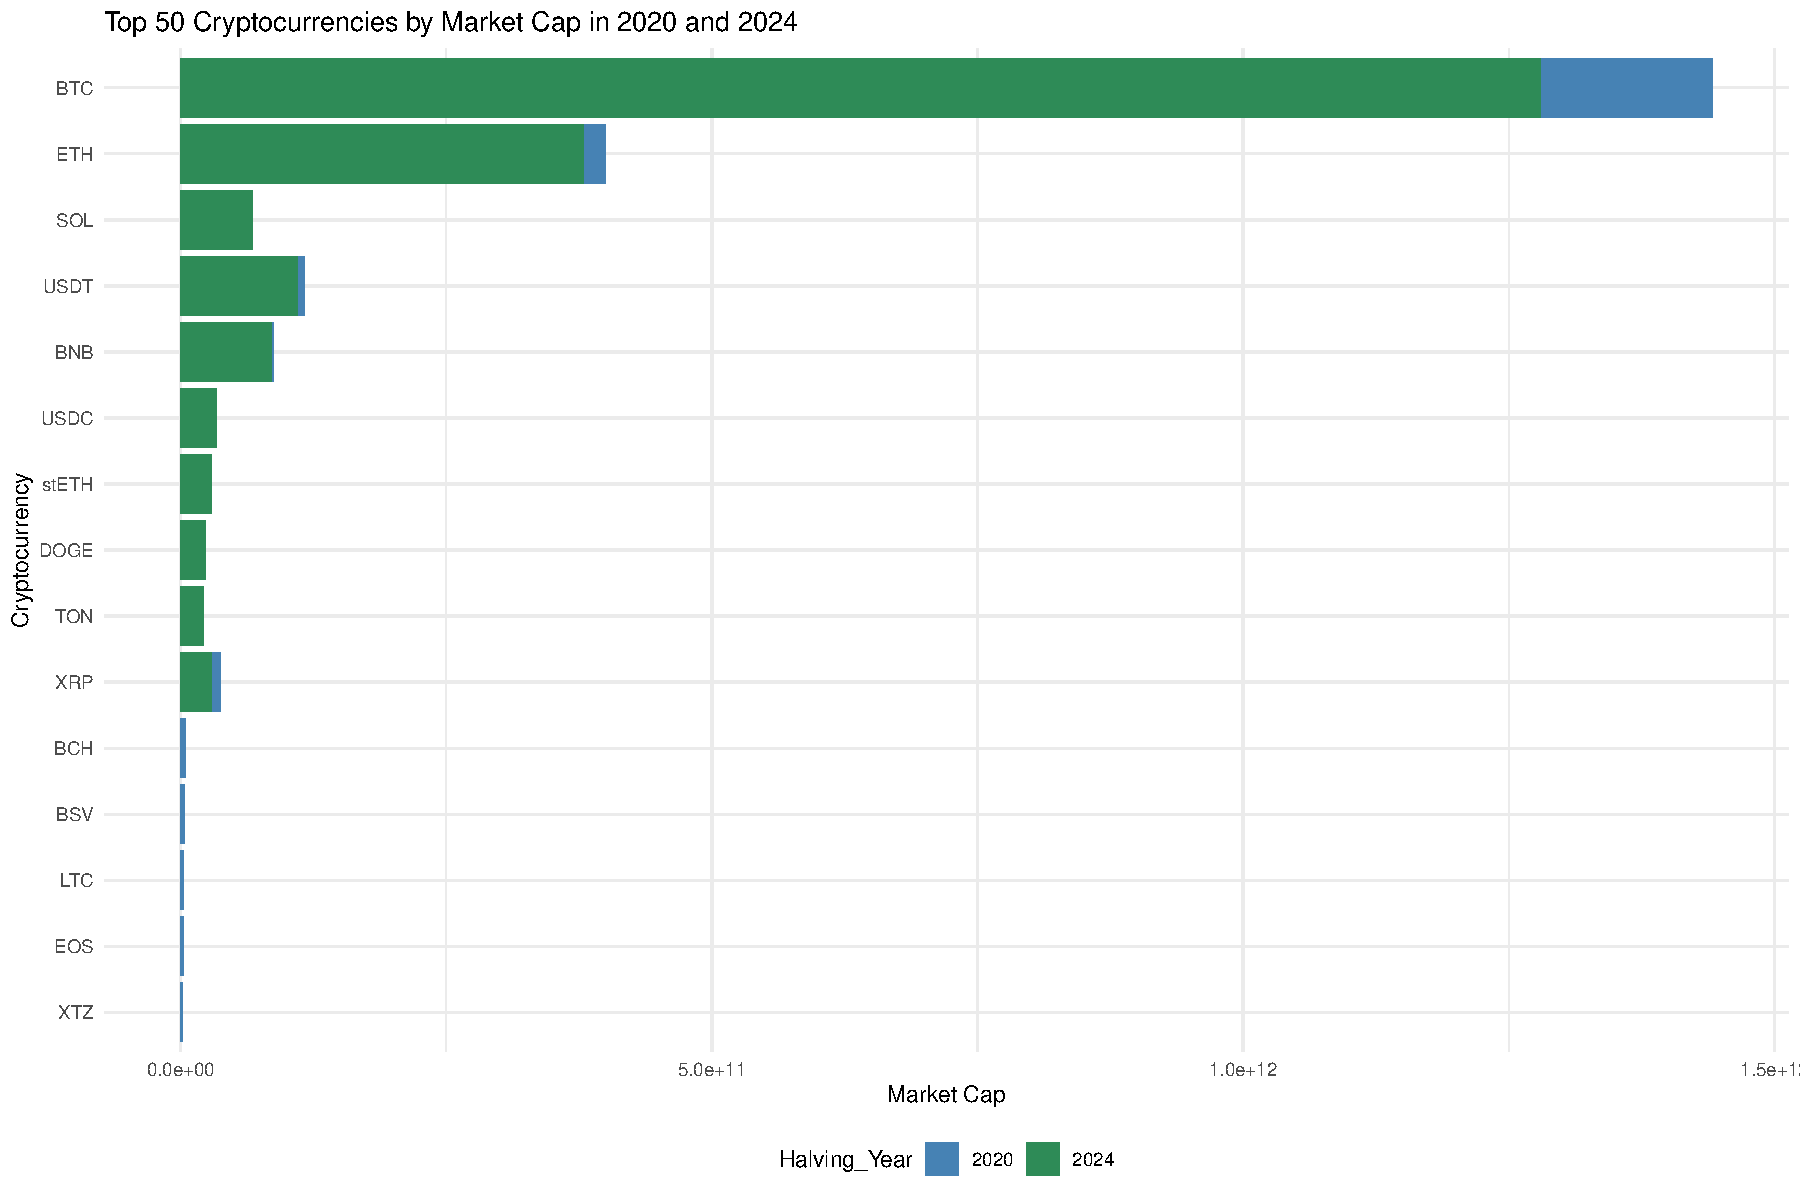
\includegraphics{Crypto_ETL_files/figure-latex/combined_halving_data top50_2020-1.pdf}

\hypertarget{market-capitalization-segmentation}{%
\section{Market Capitalization
Segmentation}\label{market-capitalization-segmentation}}

\emph{Market capitalization (market cap) is a crucial metric in the
cryptocurrency industry, representing the total value of all coins in
circulation. Its significance becomes even more pronounced around
Bitcoin halving events, a period characterized by significant
fluctuations in market cap due to the changes in block rewards.
Analyzing these fluctuations can provide investors and analysts with
critical insights into the potential gains and ideal exit points for
high-risk investments.}

\textbf{Importance of Market Cap Analysis Around Halving Dates:}

\begin{enumerate}
\def\labelenumi{\arabic{enumi}.}
\item
  \textbf{Indicator of Market Sentiment:} Market cap serves as a
  barometer for overall market sentiment and investor interest. A rising
  market cap around a halving suggests growing investor confidence and
  potential for price appreciation. Conversely, a declining market cap
  might indicate waning interest or negative sentiment, prompting
  cautious investment strategies.
\item
  \textbf{Impact of Supply Changes:} The halving reduces the rate at
  which new bitcoins are generated, directly impacting the supply side
  of the market equation. This reduced supply, if coupled with stable or
  increasing demand, can lead to a higher market cap and, by extension,
  an increase in the price per Bitcoin. Observing these dynamics helps
  predict price movements more accurately during these critical periods.
\item
  \textbf{Forecasting Future Trends:} By examining historical market cap
  trends around past halvings, investors can forecast potential
  reactions for upcoming halvings. This predictive insight is invaluable
  for formulating both short-term trading and long-term investment
  strategies.
\end{enumerate}

\textbf{Survival and Risk in Crypto Winters:} The concept of ``crypto
winters'' --- prolonged periods of low prices and reduced investor
activity --- further emphasizes the importance of market cap analysis.
During these phases, many cryptocurrencies, especially those with
smaller market caps, can fail or cease to exist. This phenomenon can be
attributed to:

\begin{itemize}
\item
  \textbf{Decreased Liquidity:} Lower market caps often result in
  reduced liquidity, making it difficult for investors to exit positions
  without impacting the price significantly.
\item
  \textbf{Funding and Operational Challenges:} Projects with lower
  valuations may struggle to secure funding or sustain operations,
  leading to their eventual collapse.
\end{itemize}

\textbf{Strategic Implications for Investors:}

\begin{enumerate}
\def\labelenumi{\arabic{enumi}.}
\item
  \textbf{Identifying Robust Investments:} Cryptocurrencies that
  maintain a stable or growing market cap through both halving events
  and crypto winters are typically more resilient and might offer safer
  investment opportunities.
\item
  \textbf{Timing Market Exits:} By recognizing patterns in market cap
  trends, investors can make informed decisions about the best times to
  exit high-risk positions, ideally before the onset of a crypto winter.
\end{enumerate}

\emph{In summary, market cap segmentation and its analysis around key
events like Bitcoin halvings and during crypto winters are vital for
understanding broader market dynamics. This analysis not only aids in
identifying potential gains but also in determining strategic exit
points to minimize exposure to high-risk investments, thereby optimizing
the investment portfolio's performance in the volatile cryptocurrency
market.}

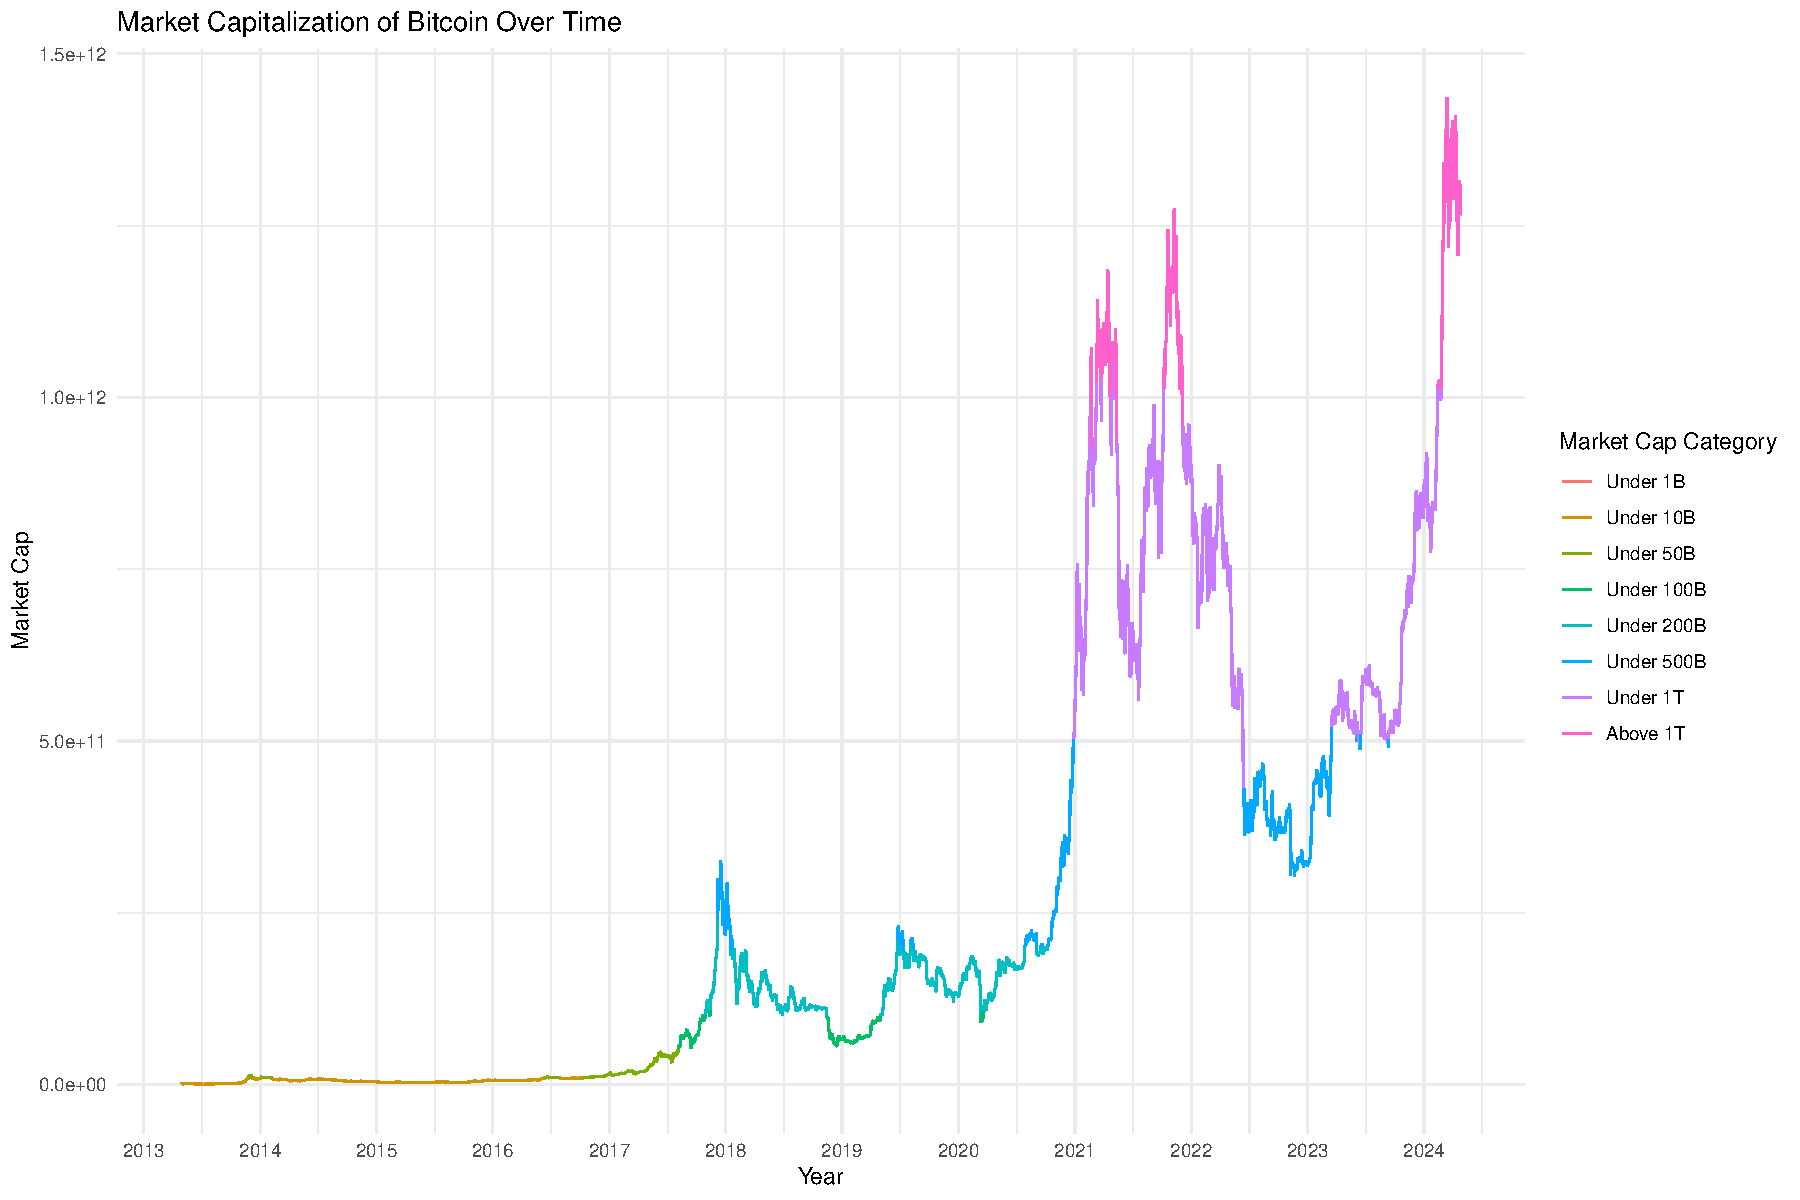
\includegraphics{Crypto_ETL_files/figure-latex/btc plot-1.pdf}

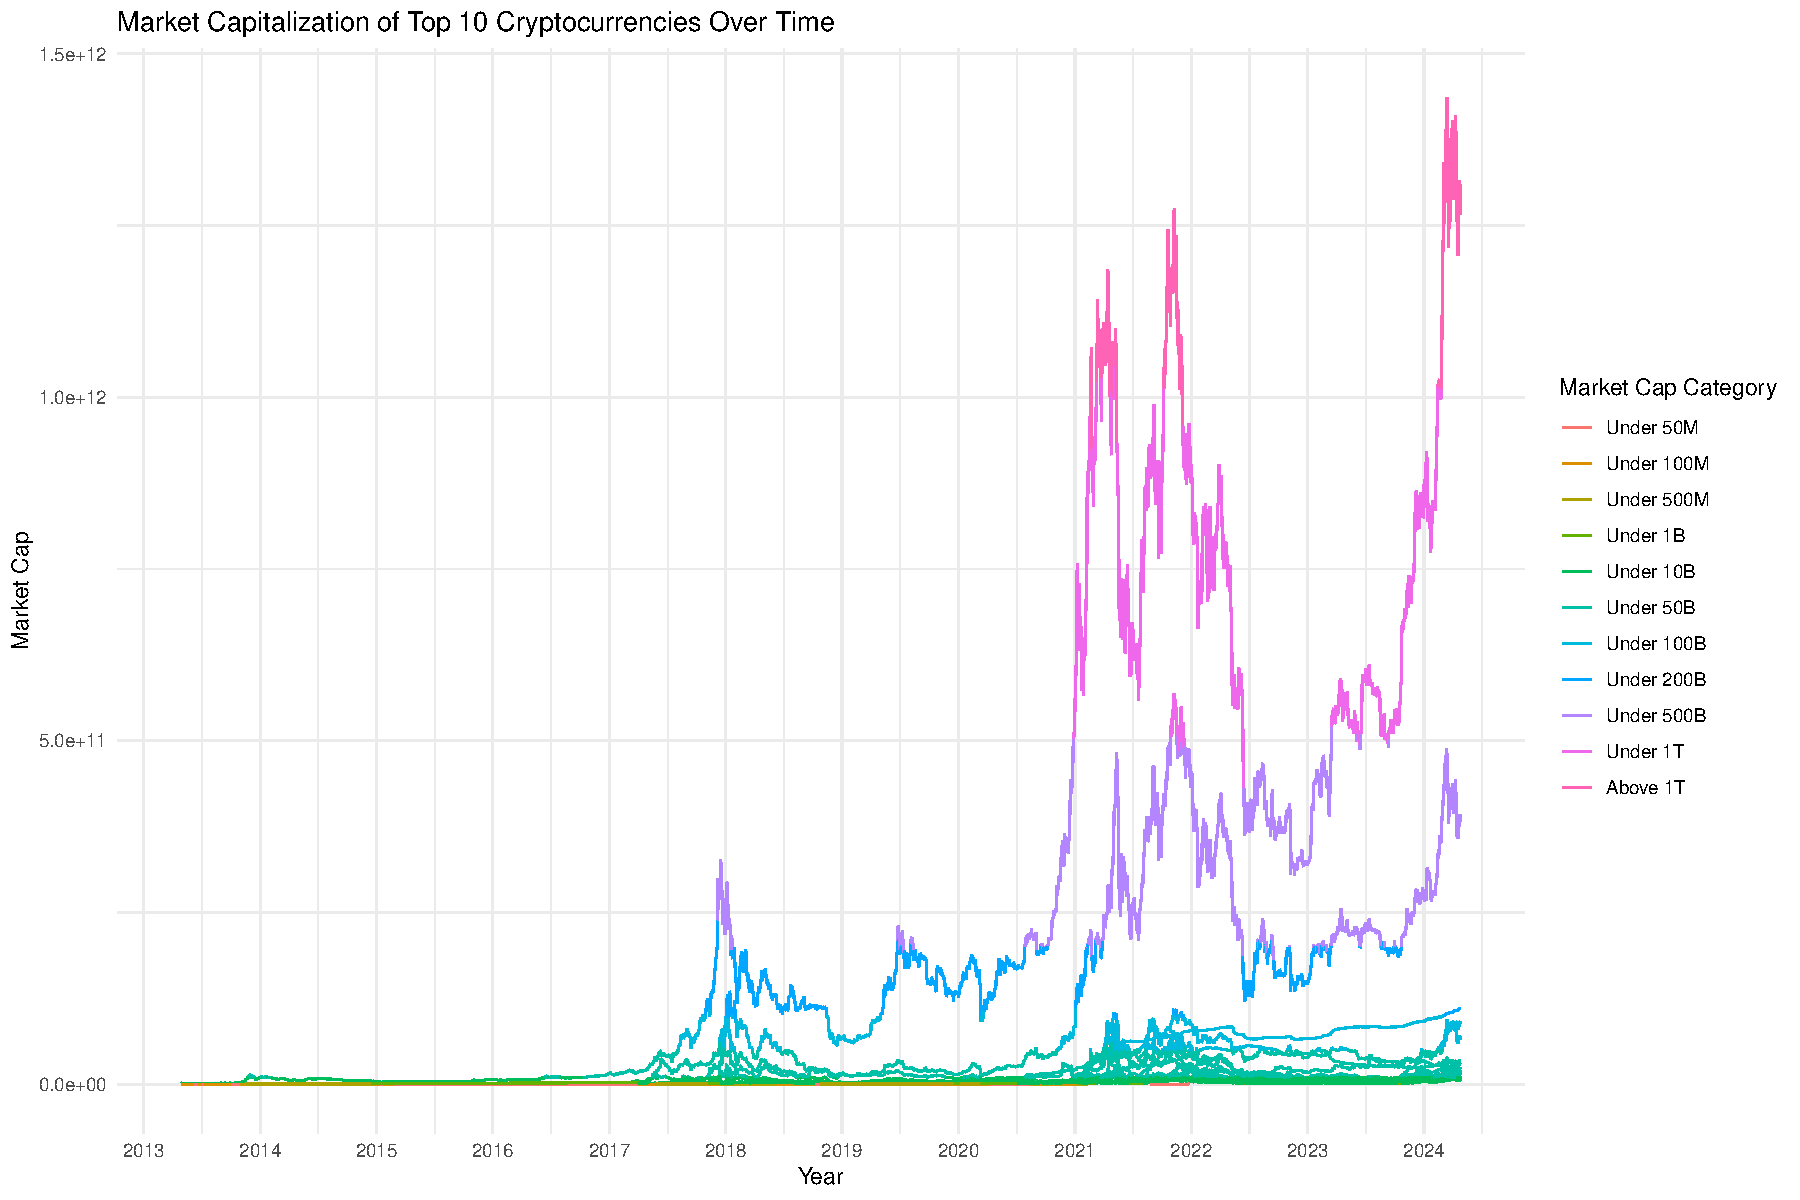
\includegraphics{Crypto_ETL_files/figure-latex/rank wise plots1-1.pdf}
\#\#\#\#\# Market Capitalization Over Time: All Top 10 Cryptocurrencies
vs.~Bitcoin: The first two plots compare the overall market cap trends
of the top 10 cryptocurrencies and Bitcoin specifically. The
visualization of Bitcoin shows more pronounced growth phases and
stabilizations, indicating its dominant and less volatile role compared
to other cryptocurrencies which have more fluctuating trajectories. This
can suggest a lower risk in Bitcoin compared to other, less established
cryptocurrencies.

\hypertarget{market-capitalization-by-rank-category}{%
\subparagraph{Market Capitalization by Rank
Category:}\label{market-capitalization-by-rank-category}}

\begin{verbatim}
    Diverse Ranks: The third plot shows market cap across different rank categories, revealing how cryptocurrencies of different market standings (e.g., top 10, top 100) behave over time. Higher-ranked cryptocurrencies (Rank 1-10) show substantial and more stable growth compared to lower-ranked categories, which display more volatility and several peaks and troughs, indicating higher risk but also potentially higher returns if timed correctly.
\end{verbatim}

\hypertarget{market-cap-vs.-log-returns}{%
\subparagraph{Market Cap vs.~Log
Returns:}\label{market-cap-vs.-log-returns}}

\begin{verbatim}
    Risk and Return Analysis: The final plot uses log returns to illustrate the potential returns against market caps across various ranks. The visual clustering of higher returns in specific market cap segments (notably in the top ranks) highlights areas of higher profitability but also underlines the higher volatility and thus higher risk.
\end{verbatim}

\hypertarget{key-points-emphasized}{%
\subparagraph{Key Points Emphasized:}\label{key-points-emphasized}}

\begin{verbatim}
*Risk Assessment*: The plots clearly categorize cryptocurrencies into segments based on their market cap, highlighting that lower market cap segments, while offering high returns, come with significantly higher risk. This is evident from the wider spreads in log returns, suggesting higher volatility.
*Return Profiles*: Higher market cap categories, especially those consistently above $1 billion, tend to offer more stable and reliable returns, appealing to risk-averse investors.
*Preliminary Analysis Disclaimer*: These visualizations serve as an initial exploration into the dynamics of the cryptocurrency market. While they provide valuable insights, they are just the starting point. A more in-depth analysis would involve statistical testing, further segmentation, integration of external factors like market conditions and regulatory changes, and potentially predictive modeling to forecast future trends.
\end{verbatim}

\hypertarget{summary}{%
\subparagraph{Summary:}\label{summary}}

The insights derived from these visualizations are instrumental for
investors to understand where the higher risks and returns lie within
the cryptocurrency market. This analysis not only informs investment
decisions but also sets the stage for deeper, more detailed explorations
to validate these initial findings.
\includegraphics{Crypto_ETL_files/figure-latex/rank wise plots2-1.pdf}

\includegraphics{Crypto_ETL_files/figure-latex/unnamed-chunk-6-1.pdf}

\begin{Shaded}
\begin{Highlighting}[]
\FunctionTok{library}\NormalTok{(ggplot2)}
\FunctionTok{library}\NormalTok{(dplyr)}

\CommentTok{\# Assuming \textquotesingle{}volume\textquotesingle{} exists and is a measure of trading volume or another metric}
\CommentTok{\# Ensure \textquotesingle{}date\textquotesingle{} is in a date format, convert if necessary}
\NormalTok{Mcapdf}\SpecialCharTok{$}\NormalTok{date }\OtherTok{\textless{}{-}} \FunctionTok{as.Date}\NormalTok{(Mcapdf}\SpecialCharTok{$}\NormalTok{date)}

\CommentTok{\# Filter the data for the specified rank ranges and prepare it for plotting}
\NormalTok{top\_coins\_data }\OtherTok{\textless{}{-}}\NormalTok{ Mcapdf }\SpecialCharTok{\%\textgreater{}\%}
  \FunctionTok{filter}\NormalTok{(rank }\SpecialCharTok{\textgreater{}=} \DecValTok{1} \SpecialCharTok{\&}\NormalTok{ rank }\SpecialCharTok{\textless{}=} \DecValTok{1000}\NormalTok{) }\SpecialCharTok{\%\textgreater{}\%}
  \FunctionTok{mutate}\NormalTok{(}\AttributeTok{rank\_category =} \FunctionTok{case\_when}\NormalTok{(}
\NormalTok{    rank }\SpecialCharTok{\textgreater{}=} \DecValTok{1} \SpecialCharTok{\&}\NormalTok{ rank }\SpecialCharTok{\textless{}=} \DecValTok{10} \SpecialCharTok{\textasciitilde{}} \StringTok{"Rank 1{-}10"}\NormalTok{,}
\NormalTok{    rank }\SpecialCharTok{\textgreater{}=} \DecValTok{20} \SpecialCharTok{\&}\NormalTok{ rank }\SpecialCharTok{\textless{}=} \DecValTok{100} \SpecialCharTok{\textasciitilde{}} \StringTok{"Rank 20{-}100"}\NormalTok{,}
\NormalTok{    rank }\SpecialCharTok{\textgreater{}=} \DecValTok{100} \SpecialCharTok{\&}\NormalTok{ rank }\SpecialCharTok{\textless{}=} \DecValTok{350} \SpecialCharTok{\textasciitilde{}} \StringTok{"Rank 100{-}350"}\NormalTok{,}
\NormalTok{    rank }\SpecialCharTok{\textgreater{}=} \DecValTok{350} \SpecialCharTok{\&}\NormalTok{ rank }\SpecialCharTok{\textless{}=} \DecValTok{1000} \SpecialCharTok{\textasciitilde{}} \StringTok{"Rank 350{-}1000"}
\NormalTok{  )) }\SpecialCharTok{\%\textgreater{}\%}
  \FunctionTok{filter}\NormalTok{(}\SpecialCharTok{!}\FunctionTok{is.na}\NormalTok{(rank\_category))}
\end{Highlighting}
\end{Shaded}

\includegraphics{Crypto_ETL_files/figure-latex/unnamed-chunk-8-1.pdf}

\begin{verbatim}
## 
## Attaching package: 'scales'
\end{verbatim}

\begin{verbatim}
## The following object is masked from 'package:readr':
## 
##     col_factor
\end{verbatim}

\begin{Shaded}
\begin{Highlighting}[]
\CommentTok{\# Create a scatter plot}
\NormalTok{scatter\_plot }\OtherTok{\textless{}{-}} \FunctionTok{ggplot}\NormalTok{(filtered\_data, }\FunctionTok{aes}\NormalTok{(}\AttributeTok{x =}\NormalTok{ cum\_log\_ret, }\AttributeTok{y =}\NormalTok{ market\_cap, }\AttributeTok{color =}\NormalTok{ mcapcat, }\AttributeTok{size =}\NormalTok{ market\_cap)) }\SpecialCharTok{+}
  \FunctionTok{geom\_point}\NormalTok{(}\AttributeTok{alpha =} \FloatTok{0.6}\NormalTok{) }\SpecialCharTok{+}  \CommentTok{\# Adjust transparency for better visibility}
  \FunctionTok{scale\_x\_continuous}\NormalTok{(}\AttributeTok{limits =} \FunctionTok{c}\NormalTok{(}\SpecialCharTok{{-}}\DecValTok{5}\NormalTok{, }\DecValTok{10}\NormalTok{)) }\SpecialCharTok{+}  \CommentTok{\# Extend the x{-}axis range to 20}
  \FunctionTok{scale\_y\_log10}\NormalTok{(}\AttributeTok{labels =} \FunctionTok{label\_scientific}\NormalTok{(}\AttributeTok{accuracy =} \DecValTok{1}\NormalTok{)) }\SpecialCharTok{+}  \CommentTok{\# Log scale for market cap with custom labels}
  \FunctionTok{scale\_color\_brewer}\NormalTok{(}\AttributeTok{palette =} \StringTok{"Dark2"}\NormalTok{) }\SpecialCharTok{+}  \CommentTok{\# A color palette that provides good contrast}
  \FunctionTok{labs}\NormalTok{(}
    \AttributeTok{title =} \StringTok{"Market Cap vs. Cumulative Log Returns for Cryptocurrencies (HD2024)"}\NormalTok{,}
    \AttributeTok{x =} \StringTok{"Cumulative Log Return"}\NormalTok{,}
    \AttributeTok{y =} \StringTok{"Market Capitalization"}\NormalTok{,}
    \AttributeTok{color =} \StringTok{"Market Cap Category"}\NormalTok{,}
    \AttributeTok{size =} \StringTok{"Market Cap"}
\NormalTok{  ) }\SpecialCharTok{+}
  \FunctionTok{theme\_minimal}\NormalTok{() }\SpecialCharTok{+}
  \FunctionTok{theme}\NormalTok{(}
    \AttributeTok{plot.background =} \FunctionTok{element\_rect}\NormalTok{(}\AttributeTok{fill =} \StringTok{"black"}\NormalTok{, }\AttributeTok{color =} \StringTok{"black"}\NormalTok{), }\CommentTok{\# Set the plot background to black}
    \AttributeTok{panel.background =} \FunctionTok{element\_rect}\NormalTok{(}\AttributeTok{fill =} \StringTok{"black"}\NormalTok{, }\AttributeTok{color =} \StringTok{"black"}\NormalTok{), }\CommentTok{\# Set the panel background to black}
    \AttributeTok{text =} \FunctionTok{element\_text}\NormalTok{(}\AttributeTok{color =} \StringTok{"white"}\NormalTok{), }\CommentTok{\# Change text color to white for visibility}
    \AttributeTok{axis.text =} \FunctionTok{element\_text}\NormalTok{(}\AttributeTok{color =} \StringTok{"white"}\NormalTok{), }\CommentTok{\# Change axis text color to white}
    \AttributeTok{axis.title =} \FunctionTok{element\_text}\NormalTok{(}\AttributeTok{color =} \StringTok{"white"}\NormalTok{), }\CommentTok{\# Change axis title color to white}
    \AttributeTok{legend.title =} \FunctionTok{element\_text}\NormalTok{(}\AttributeTok{color =} \StringTok{"white"}\NormalTok{), }\CommentTok{\# Change legend title color to white}
    \AttributeTok{legend.text =} \FunctionTok{element\_text}\NormalTok{(}\AttributeTok{color =} \StringTok{"white"}\NormalTok{) }\CommentTok{\# Change legend text color to white}
\NormalTok{  ) }\SpecialCharTok{+}
  \FunctionTok{theme}\NormalTok{(}
    \AttributeTok{axis.text.y =} \FunctionTok{element\_text}\NormalTok{(}\AttributeTok{angle =} \DecValTok{0}\NormalTok{)  }\CommentTok{\# Ensure y{-}axis labels are not angled}
\NormalTok{  )}

\CommentTok{\# Print the scatter plot}
\FunctionTok{print}\NormalTok{(scatter\_plot)}
\end{Highlighting}
\end{Shaded}

\begin{verbatim}
## Warning in scale_y_log10(labels = label_scientific(accuracy = 1)): log-10
## transformation introduced infinite values.
\end{verbatim}

\begin{verbatim}
## Warning in RColorBrewer::brewer.pal(n, pal): n too large, allowed maximum for palette Dark2 is 8
## Returning the palette you asked for with that many colors
\end{verbatim}

\begin{verbatim}
## Warning: Removed 13 rows containing missing values or values outside the scale range
## (`geom_point()`).
\end{verbatim}

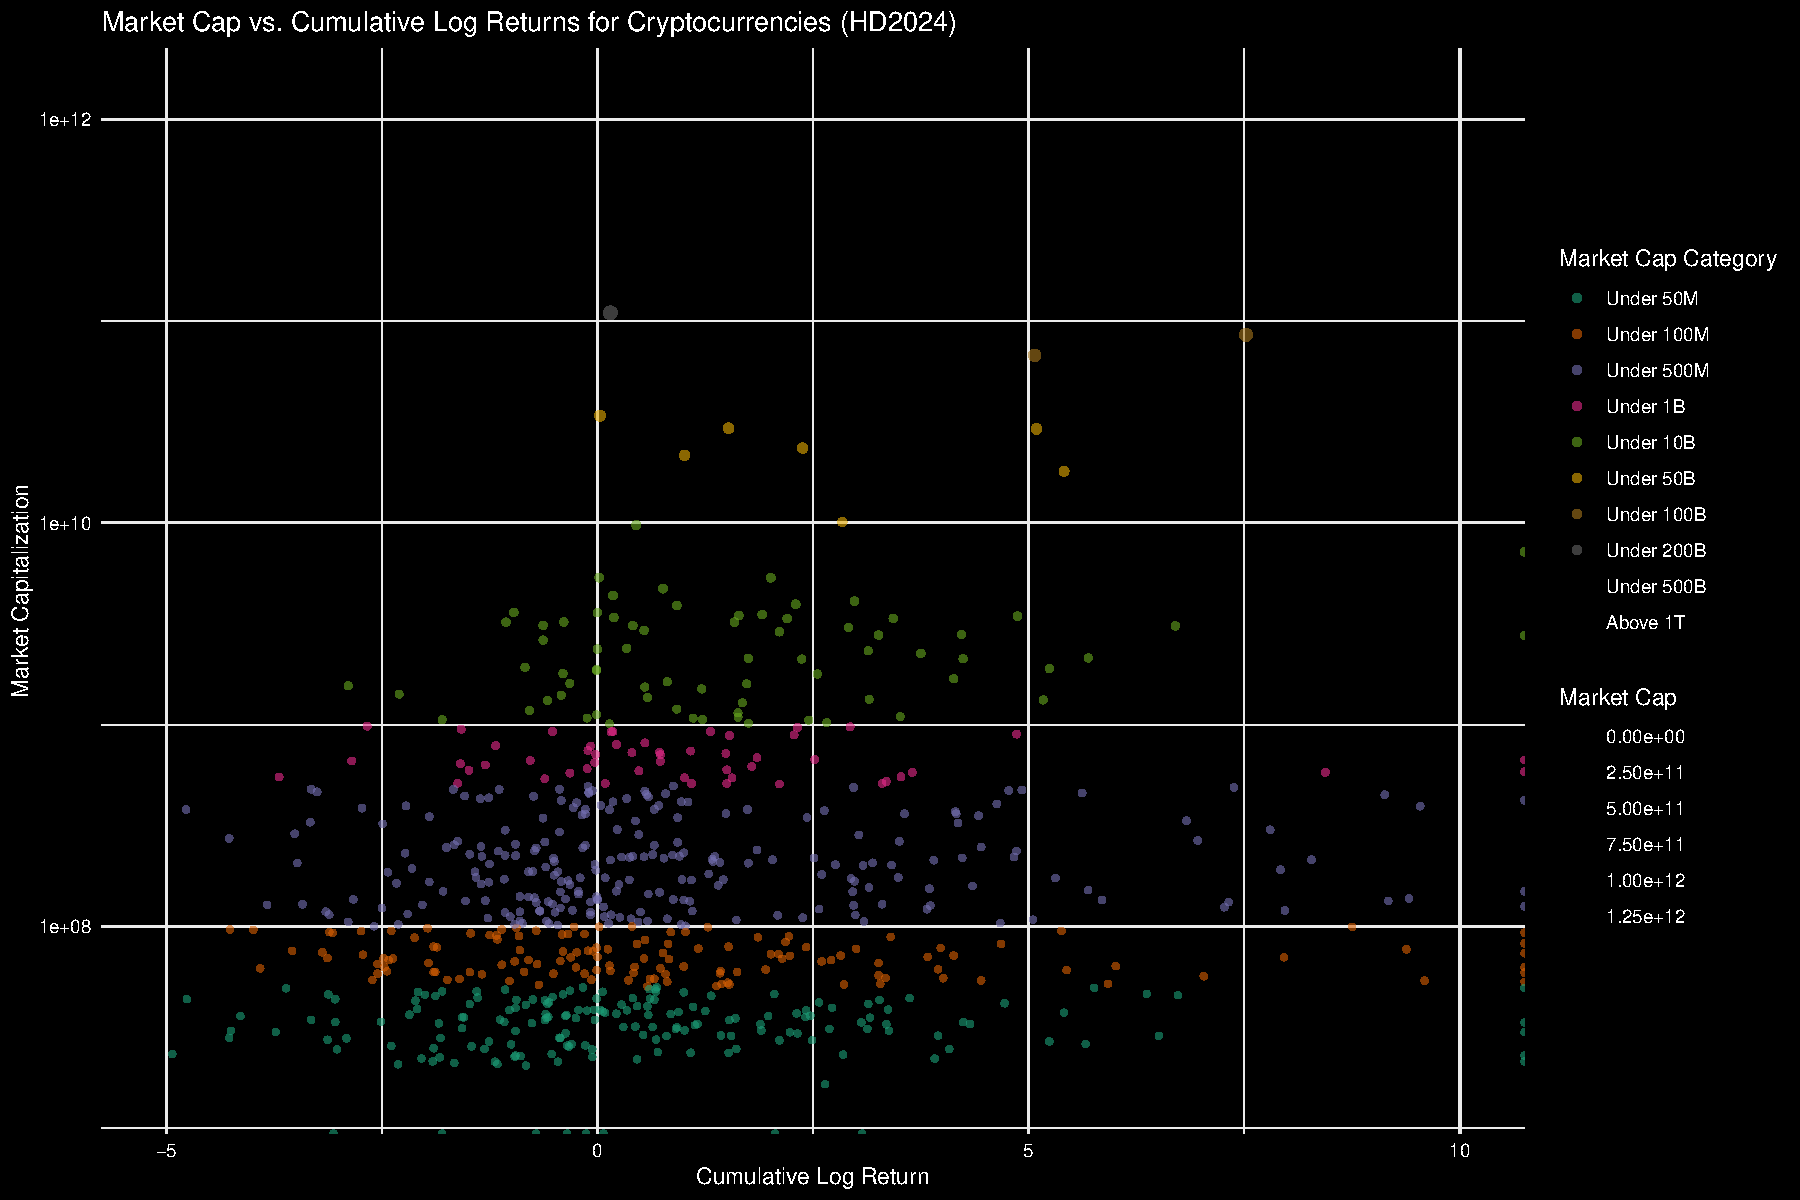
\includegraphics{Crypto_ETL_files/figure-latex/unnamed-chunk-10-1.pdf}

\begin{Shaded}
\begin{Highlighting}[]
\CommentTok{\# Create a scatter plot}
\NormalTok{scatter\_plot }\OtherTok{\textless{}{-}} \FunctionTok{ggplot}\NormalTok{(filtered\_data, }\FunctionTok{aes}\NormalTok{(}\AttributeTok{x =}\NormalTok{ cum\_log\_ret, }\AttributeTok{y =}\NormalTok{ market\_cap, }\AttributeTok{color =}\NormalTok{ mcapcat, }\AttributeTok{size =}\NormalTok{ market\_cap)) }\SpecialCharTok{+}
  \FunctionTok{geom\_point}\NormalTok{(}\AttributeTok{alpha =} \FloatTok{0.6}\NormalTok{) }\SpecialCharTok{+}  \CommentTok{\# Adjust transparency for better visibility}
  \FunctionTok{scale\_x\_continuous}\NormalTok{(}\AttributeTok{limits =} \FunctionTok{c}\NormalTok{(}\SpecialCharTok{{-}}\DecValTok{5}\NormalTok{, }\DecValTok{10}\NormalTok{)) }\SpecialCharTok{+}  \CommentTok{\# Extend the x{-}axis range to 20}
  \FunctionTok{scale\_y\_log10}\NormalTok{(}\AttributeTok{labels =} \FunctionTok{label\_scientific}\NormalTok{(}\AttributeTok{accuracy =} \DecValTok{1}\NormalTok{)) }\SpecialCharTok{+}  \CommentTok{\# Log scale for market cap with custom labels}
  \FunctionTok{scale\_color\_brewer}\NormalTok{(}\AttributeTok{palette =} \StringTok{"Spectral"}\NormalTok{) }\SpecialCharTok{+}  \CommentTok{\# A color palette that provides good contrast}
  \FunctionTok{labs}\NormalTok{(}
    \AttributeTok{title =} \StringTok{"Market Cap vs. Cumulative Log Returns for Cryptocurrencies (HD2024)"}\NormalTok{,}
    \AttributeTok{x =} \StringTok{"Cumulative Log Return"}\NormalTok{,}
    \AttributeTok{y =} \StringTok{"Market Capitalization"}\NormalTok{,}
    \AttributeTok{color =} \StringTok{"Market Cap Category"}\NormalTok{,}
    \AttributeTok{size =} \StringTok{"Market Cap"}
\NormalTok{  ) }\SpecialCharTok{+}
  \FunctionTok{theme\_minimal}\NormalTok{() }\SpecialCharTok{+}
  \FunctionTok{theme}\NormalTok{(}
    \AttributeTok{plot.background =} \FunctionTok{element\_rect}\NormalTok{(}\AttributeTok{fill =} \StringTok{"black"}\NormalTok{, }\AttributeTok{color =} \StringTok{"black"}\NormalTok{), }\CommentTok{\# Set the plot background to black}
    \AttributeTok{panel.background =} \FunctionTok{element\_rect}\NormalTok{(}\AttributeTok{fill =} \StringTok{"black"}\NormalTok{, }\AttributeTok{color =} \StringTok{"black"}\NormalTok{), }\CommentTok{\# Set the panel background to black}
    \AttributeTok{text =} \FunctionTok{element\_text}\NormalTok{(}\AttributeTok{color =} \StringTok{"white"}\NormalTok{), }\CommentTok{\# Change text color to white for visibility}
    \AttributeTok{axis.text =} \FunctionTok{element\_text}\NormalTok{(}\AttributeTok{color =} \StringTok{"white"}\NormalTok{), }\CommentTok{\# Change axis text color to white}
    \AttributeTok{axis.title =} \FunctionTok{element\_text}\NormalTok{(}\AttributeTok{color =} \StringTok{"white"}\NormalTok{), }\CommentTok{\# Change axis title color to white}
    \AttributeTok{legend.title =} \FunctionTok{element\_text}\NormalTok{(}\AttributeTok{color =} \StringTok{"white"}\NormalTok{), }\CommentTok{\# Change legend title color to white}
    \AttributeTok{legend.text =} \FunctionTok{element\_text}\NormalTok{(}\AttributeTok{color =} \StringTok{"white"}\NormalTok{) }\CommentTok{\# Change legend text color to white}
\NormalTok{  )}\SpecialCharTok{+}
  \FunctionTok{theme}\NormalTok{(}
    \AttributeTok{axis.text.y =} \FunctionTok{element\_text}\NormalTok{(}\AttributeTok{angle =} \DecValTok{0}\NormalTok{)  }\CommentTok{\# Ensure y{-}axis labels are not angled}
\NormalTok{  )}

\CommentTok{\# Print the scatter plot}
\FunctionTok{print}\NormalTok{(scatter\_plot)}
\end{Highlighting}
\end{Shaded}

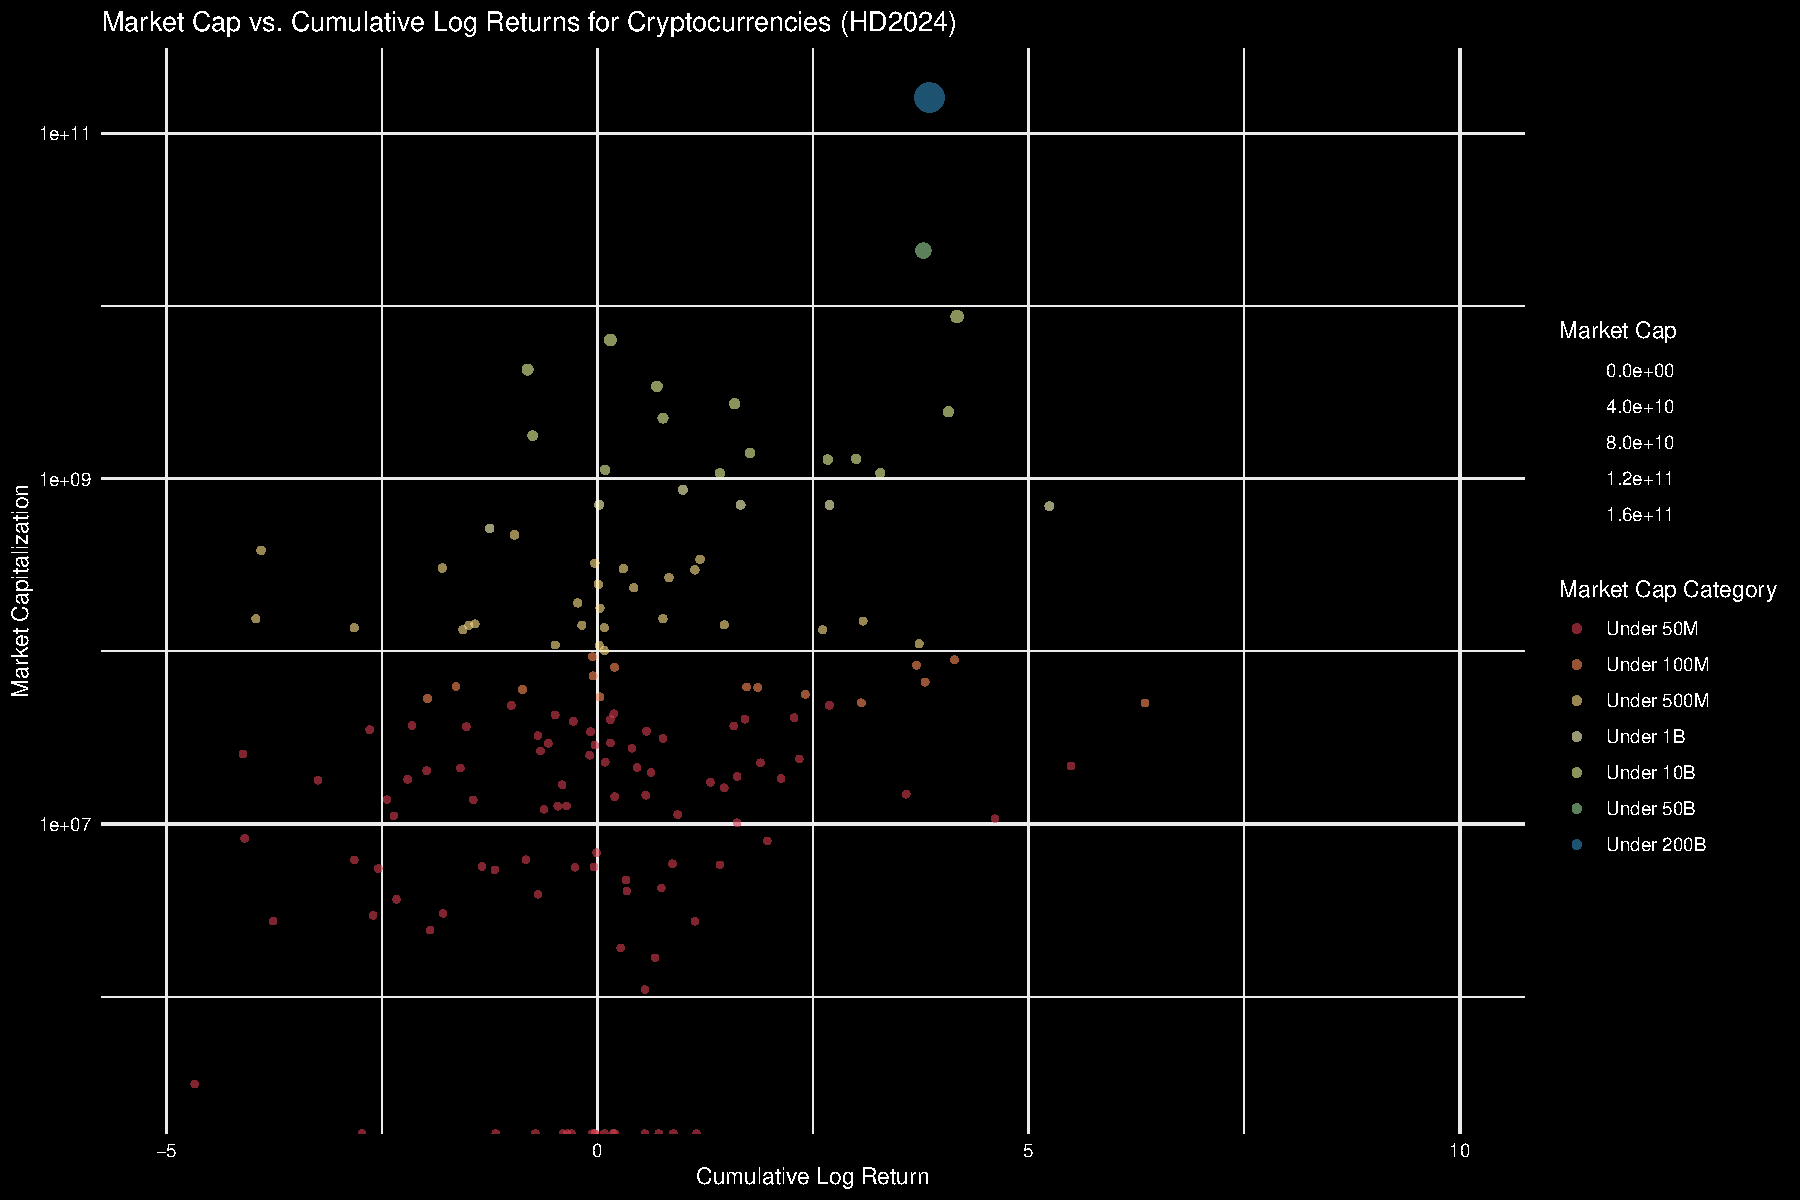
\includegraphics{Crypto_ETL_files/figure-latex/unnamed-chunk-12-1.pdf}

\end{document}
